\chapter[Discussion sur les grammaires]{Discussion sur les grammaires\\
	\LARGE{Les inventaires : \textit{R}-ance}} \label{chap:metagram}
\epigraph{\href{https://www.youtube.com/watch?v=uOHguUMnQkQ}{{\thaifont เสียงรัว ปุ่มเหงือก}}}

Ce dernier chapitre de la thèse ouvre plus largement la discussion sur la place des grammaires dans les représentations linguistiques des phones, des phonèmes, de leurs distributions, et de leurs utilisations pour des questions de recherches typologiques.

Ce chapitre s'articule en trois sections. La première section met en évidence la gageure que représentent des descriptions phonétique et phonémique d'une langue. Ces descriptions font l'objet de chapitre(s) dans les grammaires, mais comme il ne s'agit pas d'une tâche facile, il existe forcément des problèmes. La deuxième section de ce chapitre énumère les principaux problèmes que l'on trouve dans les descriptions des grammaires. Ces deux sections posent le problème de la complexité de l'interprétation des grammaires pour rendre comparable l'information qu'elles contiennent. La dernière section cherche à donner des pistes de réflexion pour l'interprétation des rhotiques dans les grammaires à travers des langues où la rhotique reportée est un trill, et des grammaires où la rhotique reportée n'est pas un trill. Nous souhaitons caractériser les \textg{trills} et les autres rhotiques à partir des grammaires. Nous donnons ensuite des exemples de processus phonologiques illustrant la difficulté de cette caractérisation.

\section{L'art de décrire un système phonétique et phonémique dans une grammaire}

Le recherche d'informations comparables dans des grammaires requiert de comprendre ce qu'est une grammaire, les informations qu'elle peut et ne peut pas apporter.
La grammaire est le résultat du travail du linguiste qui s'est déplacé sur le terrain. Elle reflète la langue mais aussi des choix théoriques dans la description. Ainsi l'écriture d'une grammaire est un exercice à part entière.\\

Dans cette section, nous allons nous intéresser spécifiquement aux recommandations et instructions en ce qui concerne la phonétique et la phonologie segmentales dans les ouvrages de référence sur l'écriture des grammaires. La phonétique a connu un changement majeur au XXème siècle. D'abord basée uniquement sur l'écoute (historiquement,  la phonétique de terrain se faisait uniquement avec les yeux et les oreilles, et avec un cahier et un crayon \parencite[212]{maddiesonPhoneticFieldwork2001}), elle a changé pour se baser sur des instruments spécifiques et des méthodes computationnelles dans le but de capturer une plus grande variation dans l'inventaire des sons du monde.

\subsection{Le terrain en phonétique}\label{subsec:lademad}

En amont de l'écriture des grammaires, les linguistes doivent procéder à l'analyse des sons de la langue qu'ils étudient. \textcite{ladefogedPhoneticDataAnalysis2003} et \textcite{maddiesonPhoneticFieldwork2001} sur la base de leurs grandes expériences sur le terrain donnent des indications sur comment enregistrer les sons d'une langue à l'aide de différents moyens techniques avec les différents problèmes associés.\\


Tout d'abord, pour \textcite{ladefogedPhoneticDataAnalysis2003}, il est important pour décrire le système phonétique d'une langue d'en connaître la phonologie. Pour autant, il faut avoir une bonne connaissance des sons de la langue pour en comprendre sa phonologie. 
Cette problématique guide sa vision de la phonétique du terrain. Les deux disciplines se doivent d'avoir un rôle à jouer en même temps dans la description de la langue. Pour \textcite[212]{maddiesonPhoneticFieldwork2001} le linguiste de terrain doit s'intéresser à la connaissance phonétique des locuteurs qui fait partie de l'ensemble de la grammaire d'une langue. La frontière entre la phonétique de terrain et la phonologie n'est pas nette car il y a cette volonté à chercher seulement ce qui est important, ce qui relève du contraste linguistique.\\

%La notion de phonème qu'il adopte est celle de \textg{sons qui contrastent dans les mots} (p. 1), et celle d'allophones de  \textg{membres d'un phonème qui occurrent dans des contextes spécifiques} (p. 6).

\textcite{ladefogedPhoneticDataAnalysis2003} estime que l'idéal est de démarrer la description du système sonore d'une langue sur la base d'une phonologie qui aurait déjà été établie dans le passé (ou d'un dictionnaire qui permet de mettre en évidence des paires minimales), avec la possibilité d'une approche comparative de l'aire géographique pour obtenir des pistes d'analyses. Au moment d'enregistrer ses locuteurs, il faut prendre en compte que l'usage des mots à enregistrer (et donc de la prononciation) peut varier en fonction du genre de la personne enregistrée, de son âge ou encore du dialecte que cette personne parle. \textcite{maddiesonPhoneticFieldwork2001} mentionne que bien que les personnes âgées aient probablement été les plus exposées à la langue, dans certains cas leur articulation peut être problématique, notamment en raison d'une diminution des capacités motrices. L'auteur recommande d'enregistrer des jeunes locuteurs ou des locuteurs d'âge moyen et d'inclure les personnes âgées pour aider si besoin pendant les élicitations.\\

Dans le but de répondre aux standards modernes de phonétique, il est nécessaire d'enregistrer plus d'un locuteur, avec au moins six locuteurs par sexe \parencite[15]{ladefogedPhoneticDataAnalysis2003}. Pour \textcite{maddiesonPhoneticFieldwork2001}, avoir plusieurs locuteurs permet de contrôler pour les potentielles idiosyncrasies. Dans le but d'obtenir du bon matériel à analyser, \textcite{ladefogedPhoneticDataAnalysis2003} recommande d'éviter de faire lire une liste de mots aux consultants mais de privilégier l'élicitation par répétition à partir de la lingua franca ou par l'image. Finalement, pour bien transcrire en API, il faut être capable de reproduire le son. Dans cette perspective, Ladefoged estime que les cours et les ouvrages de phonétiques sont utiles. \textcite{maddiesonPhoneticFieldwork2001}, lui, se base sur des élicitations de mots à partir de traductions pour obtenir des paires minimales probables et autres phénomènes intéressants dans le but d'affiner ses élicitations.\\

\textcite[218]{maddiesonPhoneticFieldwork2001} mentionne  que la phonétique de terrain s'oriente sur deux axes : la recherche de contraste et la recherche de variation pouvant être associée à ces contrastes. Par exemple, cette variation peut se retrouver au moment de marquer l'identité de genre ou faire un focus sémantique. En ce qui concerne les contrastes, ils sont la base de l'inventaire segmental. Afin de constituer un bon ensemble de données pouvant être analysé, \textcite[220]{maddiesonPhoneticFieldwork2001} recommande de bien faire attention à tous les facteurs qui peuvent avoir un rôle dans la production du son. Cela peut être des facteurs comme la position dans la syllabe, la proximité à l'accent du mot, l’environnement vocalique ou encore le débit de parole.\\

Les recommandations de \textcite{ladefogedPhoneticDataAnalysis2003} et de \textcite{maddiesonPhoneticFieldwork2001} portent sur l'enregistrement et abordent peu la question de l'analyse et de l'interprétation de ce qui a été enregistré. Ainsi, ils ne donnent pas de directives pour la transcription. Les ouvrages de grammaticographie évoquent aussi des thématiques liées au terrain phonétique et phonologique en traitant plus profondément la question de comment transcrire et quoi transcrire.

\subsection{L'art de transcrire}

Dans son introduction à la linguistique descriptive, \textcite{gleasonIntroductionDescriptiveLinguistics1961} définit le phonème comme une classe de sons (p. 258) qui doivent être phonétiquement similaires et montrent certains patterns de distribution (p. 261).
Pour lui les \textg{phone- mes are not [...] any sort of physical reality discernible by instrumental techniques or direct observation. The phoneme cannot [...] be acoustically defined} (p. 269). Le phonème est une \textg{linguistic feature}, une sorte de modélisation des faits observables, qu'il voit comme une \textg{intellectual creation of the linguist} (p. 269).\\

\textcite{gleasonIntroductionDescriptiveLinguistics1961} mentionne que la variation dans la transcription peut rendre difficile les analyses qui en découlent. Cette variation peut venir de l'utilisation inconsistante des symboles à cause par exemple d'une ouïe qui devient plus fine à force d'exposition à la langue. Les transcriptions se font généralement à travers un alphabet comme l'API (dont \citeauthor{gleasonIntroductionDescriptiveLinguistics1961} dit que son usage se justifie par l'intérêt des linguistes pour la phonologie en dépit de la phonétique), bien que le tableau consonantique donné s'inspire de l'Americanist Phonetic Notation (p. 252) surtout en ce qui concerne les rhotiques.
Le travail de phonétique de terrain consiste principalement à de l'élicitation d'énoncés courts (car plus simple à écouter, imiter et transcrire) dans le but d'obtenir des paires minimales et vérifier les paires suspectes pour postuler l'existence de phonèmes. Ce travail permettrait de faire \textg{émerger un système} (p. 289). Peu d'intérêt est porté à la phonétique. Lorsqu'il y a de la variation dans les données, le linguiste doit être capable de situer le contexte social des productions (p. 393), puisqu'il a pour objectif le contrôle de ses données pour quantifier la variation. Chaque phonème est vu comme une distribution statistique avec un possible chevauchement sur la distribution d'un autre phonème (p. 395).
Pour \citeauthor{gleasonIntroductionDescriptiveLinguistics1961}, ce qui importe n'est pas l'étendue des distributions, mais bien les contrastes entre les phonèmes.
Ainsi, toujours selon \citeauthor{gleasonIntroductionDescriptiveLinguistics1961}, le but de l'analyse phonémique serait aussi celui de l'établissement d'un orthographe (si la langue n'en possède pas déjà un) car idéalement, la langue doit posséder un orthographe standard qui est parallèle à la transcription phonémique (p. 308).\\

\textcite{vauxIntroductionLinguisticField2003}, dans leur ouvrage pour les méthodes de linguistique de terrain, dédient un chapitre à la transcription, deux chapitres à la phonétique et deux chapitres à la phonologie. Ils argumentent dans les chapitres de phonétique la nécessité de prendre en compte la phonétique articulatoire et acoustique pour décrire les langues.
En ce qui concerne les transcriptions, les auteurs spécifient qu'il est important d'être cohérent dans ses transcriptions (p. 27). Ainsi, les linguistes ont la possibilité de transcrire leurs données avec différents systèmes de transcriptions. Parmi ces systèmes de transcriptions, on retrouve l'API, l'orthographe officiel de la langue, un système orthographique se basant sur celui de la langue dominante de l'aire géographique, ou finalement d'un système standard déjà utilisé par les académiques qui travaillent sur la langue.
Certains systèmes de transcriptions possèdent des symboles plus ou moins faciles à écrire, c'est pourquoi les linguistes ont tendance à substituer des symboles qui sont plus faciles à écrire bien que moins précis (de manière similaire à ce qu'on a vu pour le \textit{r}). Dans ce cas, les auteurs spécifient explicitement qu'il faut indiquer clairement qu'il y a eu substitution d'un segment (p. 29).\\

En ce qui concerne les transcriptions larges et étroites, \citeauthor{vauxIntroductionLinguisticField2003} (p. 30-31) mentionnent que la transcription large est similaire à la transcription phonémique, c'est-à-dire qu'elle met en avant les contrastes entre les différents sons de la langue. Ce qui n'est pas important sur ce plan peut être omis. La transcription étroite permet de rendre compte des subtilités phonétiques de la langue. Ce qui est important c'est que les auteurs ne font pas de séparation claire entre les deux types de transcriptions, mais expliquent clairement qu'il existe un spectre de transcription qui est continu et que le type de transcription dépend des besoins du linguiste (\textcite[73]{bowernLinguisticFieldwork2015} mentionne aussi ce continuum dans la transcription).
Les auteurs recommandent la transcription étroite quand c'est possible, et également de faire attention à ne pas transcrire le mot comme il devrait être mais comme il est. Les auteurs reconnaissent que  dans certains cas il peut être utile de transcrire de manière large.\\

\textg{[...] you should beware of the power of the symbol choices you make} \parencite[31]{vauxIntroductionLinguisticField2003}. Pour les transcriptions, les auteurs recommandent de se baser sur les symboles utilisés pour les phonèmes de la langue et d'ajouter si besoin des éléments phonétiques supplémentaires. Sans liste de phonèmes déjà existant dans la langue, c'est au linguiste de juger comment représenter les sons. Il n'est pas donné plus d'informations sur la représentation du son ou le choix du symbole qui correspondra le mieux au phonème. On notera que dans leurs exercices de transcriptions les auteurs utilisent le \textit{r} pour l'approximante \textit{ɹ} sans le mentionner explicitement.\\

\citeauthor{vauxIntroductionLinguisticField2003} s'opposent à \textcite{ladefogedPhoneticDataAnalysis2003} dans la mesure où ils ne recommandent pas d'imiter les réalisations de locuteurs et locutrices pour mieux transcrire. Certains des arguments qu'ils donnent sont similaires à ceux que \citeauthor{ladefogedPhoneticDataAnalysis2003} donne, comme le fait que les imitations peuvent être considérées comme bonnes par les locuteurs pour de mauvaises raisons (p. 64). Un autre danger qu'ils soulignent est le fait de se faire tromper par sa propre oreille qui considérera que le son produit est similaire à celui des locuteurs natifs alors que ce n'est pas le cas.\\

Leur chapitre de phonologie segmentale s'intéresse aux allophones et aux règles et contraintes liées à la production des différents allophones. Les auteurs expliquent qu'il existe un moment lors de l'analyse phonologique durant lequel il faut sélectionner les formes sous-jacentes et que c'est un défi \textg{intellectuel et mécanique} (p. 80). Un point clef mis en avant est que l'allophone qui va être choisi pour la forme sous-jacente doit être dans l'idéal celui à partir duquel il est le plus aisé de dériver les autres allophones à travers des règles phonologiques. Ils donnent l'exemple des allophones [t], [tʰ], [ɾ] et [tʃ] (et un autre allophone dont nous n'avons pas réussi à interpréter le symbole) qui peuvent être dérivés via peu de règles, si l'on choisit /t/ comme forme sous-jacente.\\


\textcite{chelliahHandbookDescriptiveLinguistic2011} et \textcite{bowernLinguisticFieldwork2015} consacrent un chapitre au terrain phonétique et phonologique. \citeauthor{bowernLinguisticFieldwork2015} dédie aussi des sections dans un chapitre consacré aux débuts du travail sur une langue, à la découverte de l'inventaire phonémique et à la transcription; elle y recommande l'utilisation de Praat \parencite{boersmaPRAATSystemDoing2001} pour la vérification des transcriptions. \citeauthor[41]{bowernLinguisticFieldwork2015} recommande de prendre note de toutes les difficultés que le linguiste de terrain peut avoir avec les transcriptions. \\


Pour \textcite[256]{chelliahHandbookDescriptiveLinguistic2011} le linguiste peut se permettre de transcrire largement si les systèmes phonétiques et phonologiques ont déjà été décrits par d'autres chercheurs/euses. La transcription étroite peut être utilisée pour mettre en évidence les sons qui sont encore problématiques dans la langue (ce que nous interprétons comme les sons en libre variation). Lors de la transcription, il faut être conscient des conventions de transcription utilisées, c'est-à-dire tout ce qui ne vient pas d'un système de transcription déjà établi, et qui peuvent être régionales \parencite[43]{bowernLinguisticFieldwork2015}. \citeauthor{bowernLinguisticFieldwork2015} (p. 73) considère que la transcription large est plus adaptée pour les recherches de mots et pour la description, et la recommande pour cela.

En ce qui concerne les descriptions de terrain, les propos des auteurs sont relativement similaires à ceux déjà donnés par \textcite{ladefogedPhoneticDataAnalysis2003} et \textcite{maddiesonPhoneticFieldwork2001} (mentionné en \autoref{subsec:lademad}).



%Si on parle de Laver -> je vais regarder ce qu'il dit sur la transcription
%Bowern (2008) -> donne des exemples pour la transcription phonémique c'est bien

%Model structuralist phonemic analyses to consult are: Ferguson (1960) on Bengali; Matthews (1955) on a Dakota dialect (Siouan); and Haugen (1958) on Icelandic.


%2 - Transcription 26 : 35
%Voegelin, Charles. 1960. Guide for Transcribing Unwritten Languages in Field Work. Manuscript, Harvard University
%Kelly, John and John Local. 1989. Doing phonology: observing, recording, interpreting. Manchester: Manchester University Press.
%5 - 61
%6 - 68
%7 - 77 -> 83

%Phonetic data analysis: an introduction to fieldwork and instrumental techniques - Ladefoged
%Elements of Acoustic Phonetics Ladefoged
%Introduction to linguitic field metholds - Vaux and Cooper

%Handbook of Descriptive Linguistic Fielwork - Chelliand et de Reuse

%Linguistic fieldwork - Bowern
%Bowern, Claire. 2008. Linguistic Fieldwork. A Practical Guide

\subsection{Résumé du terrain en phonétique}

D'après les indications, préalablement à un travail de terrain en phonétique, il faut déjà être suffisamment à l'aise avec les techniques d'enregistrement, la théorie sur la production de la parole, la transcription et la terminologie. \textcite{bowernLinguisticFieldwork2015} et \textcite{riceSoundsGrammarWriting2014} mentionnent que ce sont généralement des doctorant.e.s (mais pas que) qui écrivent des grammaires de langues en danger. Il faut donc prendre en compte la nature limitée des ressources financières et du temps pour le travail de thèse. \textcite{riceSoundsGrammarWriting2014} cite Noonan (2005, p. 354)\footnote{Noonan, Michael. 2005. Grammar writing for a grammar reading audience. Dans Thomas Payne \& David Weber (éditeurs invités) \textit{Studies in Language} 30.2. 351-365.}, pour qui il faut avoir des standards élevés lors de la description d'une langue.
\textcite[251]{chelliahHandbookDescriptiveLinguistic2011} vont dans le même sens en disant : \textg{so whether the goals are language documentation or language description, there is no room for sloppy phonetic fieldwork}. Il y a donc une forte pression vis-à-vis du travail de terrain en phonétique.
En ce qui concerne la collecte des données \textcite[36]{bowernLinguisticFieldwork2015} suggère de \textg{[m]ake the best of what you have at the time.}\\

%Ouvrir sur la perspective de la transcription assisté par les technologie.

Selon ces différents ouvrages, la finalité du terrain en phonétique est l'inventaire des sons, l'établissement des phonèmes et des allophones. Il ne s'agit pas de travailler sur la variation ou sur la capacité à produire des sons.

Ainsi, la finalité d'un terrain en phonétique ne tient pas dans l'écriture de sa grammaire. On ne trouve pas particulièrement d'indications sur l'écriture d'une section phonétique/phonologie dans la grammaire et sur quoi intégrer à sa grammaire. Ce qui ressort comme vraiment important ce sont les notes des carnets de terrain dans lesquelles il est recommandé aux linguistes de tout écrire (dans un premier temps).\footnote{Il pourrait être intéressant de faire une analyse des notes de linguistes et de regarder à partir de quel moment le symbole \textit{r} commence à être utilisé. Il s'agit de voir si avant un autre segment \textg{simil-r} est utilisé - sur la base de \textcite[43]{bowernLinguisticFieldwork2015} : \textg{Once you’ve come up with a transcription system, either stick to it or make sure that you make a note of the point at which you changed and the equivalences between the old system and the new; otherwise, you’ll confuse yourself and others who use your notes.}} \\

Les différents auteurs présentent le terrain en linguistique, et expliquent ce à quoi il faut faire attention et donnent des indications sur la manière de récupérer, analyser et transcrire des données. Bien que certains auteurs recommandent des transcriptions étroites, il faut cependant prendre en compte qu'elles sont plus chronophages que les transcriptions larges. Dans les deux cas, la fluidité dans la transcription vient avec l'expérience. 
\textcite{bowernLinguisticFieldwork2015} donne une liste de concepts de phonétique/phonologie à prendre en considération pour l'élaboration d'une esquisse phonologique, ce qui peut s'apparenter à une structure de chapitre de grammaire.

\section{Métagrammaticographie}

Le terme de \textg{métagrammaticographie} provient de \textcite{lehmannGrammaticography2004} et s'oppose à celui de \textg{grammaticographie} qui est l'activité s'intéressant à l'écriture des grammaires des langues. La métagrammaticographie est \textg{la recherche de principes méthodologiques qui réconcilient [la grammaticographie] avec la théorisation linguistique} (p. 1857). Il s'agit d'une \textg{réflexion théorique que l'on porte à la conception des grammaires} \parencite[p. 94]{barabyGrammaticographieLanguesMinoritaires2011}. Cela peut se faire par deux moyens : soit en procédant à l'extraction des principes grammaticographiques suivis par les linguistes, soit en inférant les pré-requis pour faire une grammaire adéquate à partir de grammaires de qualité.
La métagrammaticographie décrit les grammaires pour en faire des instructions pour l'élaboration de nouvelles grammaires. 
\citeauthor{lehmannGrammaticography2004} disent que \textg{[l]es données doivent exister indépendamment de la production de la grammaire} (p. 1860), et en ce qui concerne les analyses théoriques, les cheminements intellectuels doivent être transparents.
Les auteurs mentionnent que dans les transcriptions phonétiques, les symboles choisis proviennent de l'API, mais que lorsque le détail phonétique n'est pas important, il est possible d'opter pour des symboles moins techniques (p. 1876). Outre cette mention, la phonétique et la phonologie ne sont pas mentionnées comme des objets auxquels la métagrammaticographie doit s'intéresser, laissant plus de place à la syntaxe et à la morphologie.\\

\textcite{riceSoundsGrammarWriting2014} s'intéresse à la place des sons dans l'écriture des grammaires. Son but, à travers son regard réflexif, est de donner des indications sur ce qu'il faut inclure à propos des sons dans une grammaire à partir de ce qui se fait déjà dans les grammaires. L'autrice rappelle que les ouvrages sur l'exercice de l'écriture n'abordent pas la phonétique et la phonologie en profondeur, et qu'aucun des ouvrages qu'elle cite possèdent de \textg{detailed reflection on the role of sound in a grammar, what the issues are, and how to work through these issues} \parencite[72]{riceSoundsGrammarWriting2014}.\\

En s'intéressant aux objectifs qu'une grammaire doit remplir, \citeauthor{riceSoundsGrammarWriting2014} mentionne que généralement la phonétique et la phonologie sont reléguées au second plan après la syntaxe, la morphologie et la sémantique. Pour ce qui est de la description de langue à tradition orale et sans système d'écriture, il faut dans un premier temps être capable d'entendre et de reconnaître les sons, ce que \citeauthor{riceSoundsGrammarWriting2014} considère comme un challenge dans la mesure où la langue native de la personne qui décrit la langue peut jouer comme un filtre pour les sons qui ne sont pas natifs dans sa langue. À cela s'ajoute la nécessité de se confronter au problème de la transcription. Les linguistes doivent utiliser un système de transcription qu'il faut ensuite pouvoir décoder, ce qui n'est pas forcément le cas avec tous les symboles de l'API. L'autrice mentionne que quelque chose peut être perdu en passant du son au papier (p. 84). Bien que les transcriptions soient utiles, \citeauthor{riceSoundsGrammarWriting2014} (p. 88) remarque le fait qu'elles peuvent soulever des questions de vérifiabilité et de rigueur scientifique. \citeauthor{riceSoundsGrammarWriting2014} prend l'exemple du [t] qui peut être tantôt dental tantôt alvéolaire, et nous prenons l'exemple du [r] dont la variation a été détaillée dans les précédents chapitres. En effet, \textg{it is not uniformly the case in practice that a symbol is uniquely interpretable: the transcription itself is an abstraction} \parencite[74]{riceSoundsGrammarWriting2014}.\\

Dans son travail s'inscrivant dans la métagrammaticographie, \citeauthor{riceSoundsGrammarWriting2014} s'est intéressée à des grammaires allant de la fin du XIXème siècle à aujourd'hui.\\

L'autrice rapporte que le noyau de la phonologie incluse dans les grammaires a pu varier selon les périodes.
Dans les grammaires les plus anciennes qu'elle a étudiées, le noyau de la phonologie était constitué d'une liste des sons, de leur prononciation, de la phonotactique ainsi que d'une discussion des allophones et allomorphes se trouvant dans la langue. À ce noyau pouvaient s'ajouter des informations prosodiques et des informations sur la variation des interlocuteurs. Dans les grammaires de la deuxième moitié du XXème siècle, ce noyau est constitué d'une description des sons contrastifs, des allophones, de la morphophonémique, et peu d'attention les unités au dessus du mot comme celles appartenant à la prosodie.
Les grammaires qu'elle étudie sont mises en parallèle avec les lignes directrices de l'époque pour l'écriture de grammaires. Elle cite Comrie and Smith (1977)\footnote{Comrie, Bernard \& Norval Smith. 1977. Routledge Descriptive Grammar Series. Lingua Descriptive Studies: Questionnaire. Lingua 42. 1-71.} dans l'introduction du \textit{Routledge Descriptive Grammar Series} qui mentionnent que les exemples devraient être accompagnés des transcriptions phonétiques ou phonémiques adéquates en API, et que lorsque des valeurs différentes sont données à des symboles, il faut être explicite. Une description phonologique doit comporter de la phonologie segmentale, suprasegmentale, mais aussi des éléments de phonotactiques et de la morphophonologie. \citeauthor{riceSoundsGrammarWriting2014} mentionne aussi les lignes directrices de Dixon et Rice éditeurs dans les années 1990 pour la \textit{Cambridge University Press Grammar Series} où les phonèmes doivent être présentés sous forme de tableau avec une description des réalisations, et les allophones dans leur environnement avec les symboles API (sauf pour une bonne raison - sans préciser ce qu'est une bonne raison).\\

Les grammaires les plus récentes que \citeauthor{riceSoundsGrammarWriting2014} étudie bénéficient de l'avancée des technologies. Ainsi, beaucoup de grammaires contemporaines peuvent inclure des spectrogrammes grâce à Praat. Cependant, l'auteur souligne que les \textg{[a]coustic representations require a depth of knowledge to interpret, and they remain a representation of sound rather than sound itself} \parencite[80]{riceSoundsGrammarWriting2014}. Dans certains cas, des enregistrements audios avec les grammaires peuvent, et devraient, être disponibles en étant couplés avec des transcriptions alignées dans le temps.\\

Ainsi \citeauthor{riceSoundsGrammarWriting2014} (p. 84--85) donne les lignes directrices suivantes comme aboutissement de son travail de métagrammaticographie sur les sons dans les grammaires :
\begin{exe}
	\ex \begin{xlist}
	\ex Presentation of segmental inventories, together with articulatory descriptions and discussion of allophones and variation, with careful exemplification. 
	\ex Presentation of phonotactics and syllable structure, with careful exemplification, including discussion of any morphological factors that affect the distribution of sounds (e.g., there might be a richer inventory in stems than in affixes). In discussion of phonotactics, it is important to talk about positional inventories, including any differences in inventories that might exist depending on prosodic position.
	\ex Presentation of suprasegmentals, including tone, stress, and intonation, with careful exemplification, augmented with pitch tracks.
	\ex Presentation of phonological rules, with careful exemplification and motivation.
	\ex Phonological analyses are not always as clean as one might like – for instance, it is often difficult to decide on what is phonemic and what is not in a language and there might be sounds that are of very limited occurrence– and these types of complexities should be addressed.
	\end{xlist}
\end{exe}


Parmi ces lignes directrices, les points les plus importants qui ont guidé notre recherche dans les grammaires sont les présentations et descriptions des sons.\\

\citeauthor{riceSoundsGrammarWriting2014} (p. 85) consciente des problèmes liés au \textit{r} précise que les \textg{[r]hotics should be described in as much detail as possible, as the symbol \textit{r} is used in many different ways}. Pour elle (p. 86), il est important de mettre la variation en avant avec des informations sur la variation inter-individuelle mais aussi intra-individuelle. Les réalisations des \textit{r} varient en fonction des locuteurs/trices mais aussi en fonction des contextes phonologiques, et c'est cette variation que les grammaires devraient mettre en avant pour nuancer le \textit{r} avec une seule réalisation.\\

Il nous est apparu que l'intégration des sons dans les grammaires peut donc être problématique à tous les niveaux. Que ce soit avec l'écoute des audios, les transcriptions, et les représentations acoustiques du signal sonore, il existe des biais rendant cette tâche difficile. Cependant, c'est uniquement à travers l'intégration de ces trois niveaux ensemble et l'explicitation des choix méthodologiques et théoriques que les grammaires pourront mettre en valeur la phonologie segmentale des langues. Tant que ces conditions ne seront pas remplies, les grammaires ne seront pas un bon endroit pour investiguer les réalisations des \textg{r}.

\section{Problèmes lors de l'étude de grammaires}

\subsection{Principaux problèmes}

Dans cette section, nous allons parler plus en détails de problèmes méthodologiques qui rendent difficile la comparaison des différentes sources des langues décrites en ce qui concerne leurs sons, et donc rendent difficile l'investigation du \textit{r}.\\

Lors d'une présentation orale à un public de typologues et de linguistes de terrain, \textcite{maddiesonPhoneticAdequacyDescriptive2021} mentionne plusieurs problèmes rendant difficile (voire dans certains cas impossible) la comparaison exacte des inventaires des sons des langues.
Quatre principaux points sont abordés :
\begin{enumerate}
	\item Le manque d'information
	\item La présence de descriptions vagues, confuses ou encore ambiguës
	\item La présence de déclarations conflictuelles
	\item Le manque de documentation
\end{enumerate}

Nous illustrons certains de ces points. Par rapport au manque d'information, il prend, parmi ses exemples, celui du terme rhotique représenté par un \textit{r} dans le tableau des consonnes. Parler de \textg{rhotique} n'est pas informatif sur le son pouvant être produit (pour les raisons que nous avons aussi vues en \autoref{chap:jipa} et \autoref{chap:acoustics}). \citeauthor{maddiesonPhoneticAdequacyDescriptive2021} parle aussi du manque d'information concernant le lieu d'articulation, qui peut osciller entre dental et alvéolaire dans certains cas, ou ne pas être spécifié du tout.
Vis-à-vis de la présence de déclarations conflictuelles, \citeauthor{maddiesonPhoneticAdequacyDescriptive2021} mentionne qu'elle peuvent, entre autres, se manifester à travers des erreurs dans les symboles utilisés. Pour rappel dans le \autoref{chap:jipa}, nous avions trouvé des \textit{r} dans certaines \textit{Illustrations of the IPA} quand des \textit{ɾ} ou des \textit{ɹ} auraient été attendus. De plus, la ressemblance entre les caractères \textit{r} et \textit{ɾ} rend les erreurs propices dans les transcriptions.\\

\citeauthor{maddiesonPhoneticAdequacyDescriptive2021} tente d'expliquer l'origine de ces problèmes. Pour lui, certaines des raisons sont :
\begin{enumerate}
	\item Des problèmes existant dans les cadres théoriques (cf. la \autoref{subsec:lingtrad} pour l'Alphabet Phonétique International)
	\item Une terminologie ambiguë avec l'utilisation de \textg{cover terms}. Par exemple, l'utilisation de termes comme \textg{rhotique} et \textg{vibrant} rendent difficile l'interprétation des réalisations phonétiques.
	\item Une orientation spécifique au terrain 
	\item Un manque de formation phonétique (ou phonologique). Cela s'explique par un manque d'opportunité d'entraînement aux études phonétiques et un manque d'intérêt pour le domaine. Dans beaucoup de cas, développer une orthographe pratique pour décrire la langue est une priorité pour la personne qui décrit la langue.
	\item Un focus principal sur la morphologie et la syntaxe.
\end{enumerate}

\textcite{maddiesonPhoneticAdequacyDescriptive2021} recommande donc de faire attention à la terminologie utilisée, et de travailler en collaboration avec des phonéticiens lors de la description d'une langue. Il faut inclure des analyses phonétiques aux grammaires et rendre disponibles les enregistrements sonores.

%Ces informations et pistes de réflexion sont importantes car elle s'applique à la réflexion critique qu'il faut porter à notre révision des grammaires pour la réplication l'étude crosslinguistique de \textcite{winterTrilledAssociatedRoughness2022}.

\subsection{Corpus multi-lingues et multi-alphabets}


Pour \citeauthor{haspelmathComparativeConceptsDescriptive2010} \parencite*{haspelmathComparativeConceptsDescriptive2010,haspelmathChallengeMakingLanguage2016}, une langue doit être décrite avec ses propres concepts.  Mais si une langue doit être écrite avec ses propres concepts, cela ne donne aucune indication sur la langue de rédaction de sa description. 
Il existe en effet une grande hétérogénéité dans les langues choisies pour la description. Bien que l'anglais soit la langue principale de rédaction, ce n'est pas la seule. 
Ainsi, il est possible de retrouver de l'indonésien pour décrire les langues parlées en Indonésie, du Russe pour les langues parlées dans les pays de l'ex-URSS, de l'espagnol pour les grammaires des langues d'Amérique Centrale et Latine, du portugais pour les langues du Brésil ou d'autres anciennes colonies portugaises comme Timor-Leste, ou du français pour certaines grammaires de langues de pays d'Afrique francophone. Ce ne sont que des exemples, et ils ne sont pas uniques. Lors du re-codage des données pour la réplication de l'étude cross-linguistique de \textcite{winterTrilledAssociatedRoughness2022} nous avons dû travailler avec des grammaires écrites en chinois, en allemand, en finnois, en norvégien, en hongrois ou encore en suédois.\\

La technologie est notre alliée et permet, dans une certaine mesure, de remédier au problème de la pluralité des langues. Pour notre re-codage, nous avions fait le choix de garder les grammaires et les sources écrites dans des langues ou scripts/alphabets que nous ne maîtrisions pas car la technologie est telle qu'il est possible de faire des traductions automatiques. Pour cela, nous avions utilisé \texttt{Google Lens} à partir de l'application \texttt{GoogleTraduction} (\texttt{Version 6.36.1}) en utilisant la caméra d'un iPhone 12mini pour traduire automatiquement ce que nous n'étions pas en mesure de lire ou de comprendre (Figure \ref{fig:couvgt}), ou nous avons utilisé la version gratuite de DeepL lorsque nous le pouvions.

\begin{figure}
	\centering
	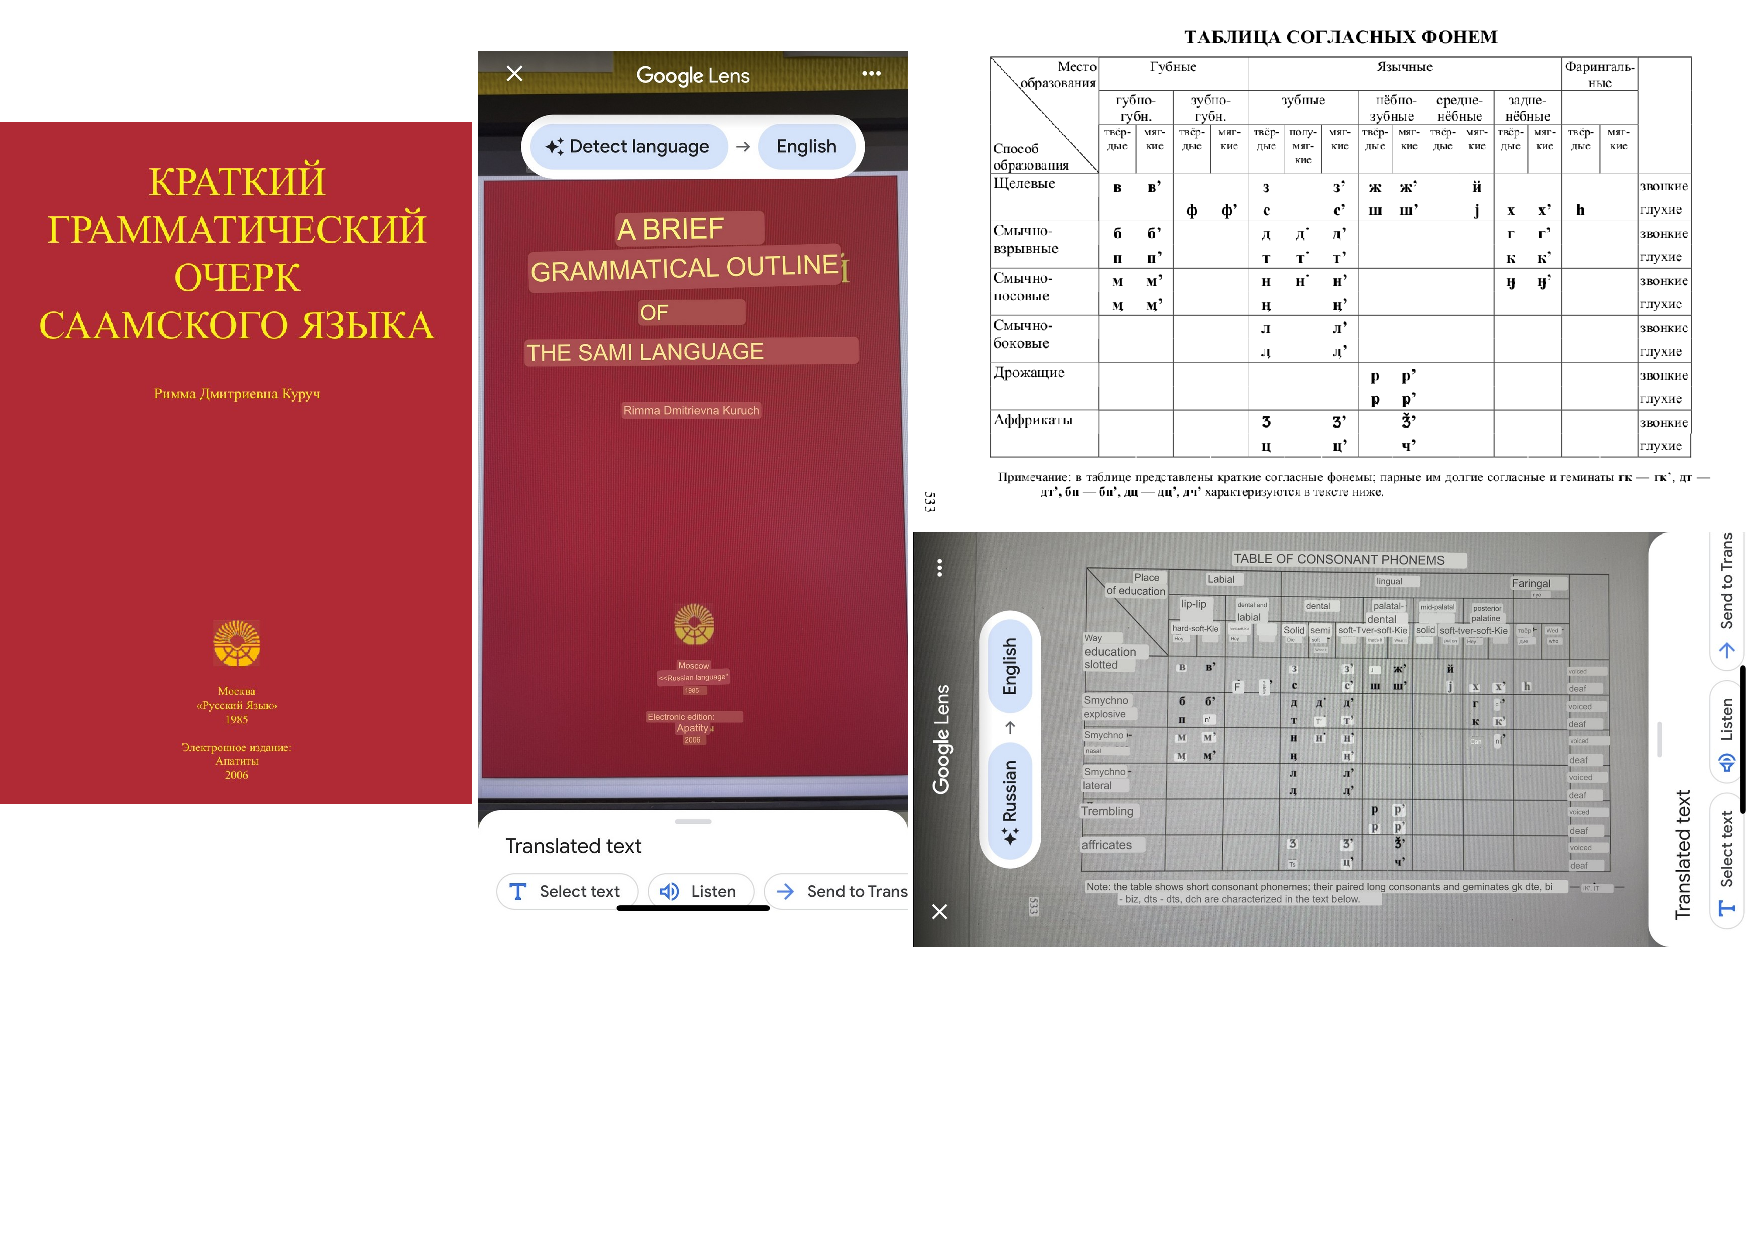
\includegraphics[width=1\linewidth,
	trim={0 5cm 0 0}, clip]{substance/images/CouvGT}
	\caption[Exemple d'utilisation de \texttt{Google Lens}]{Exemple d'utilisation de \texttt{Google Lens}. Дрожащие est traduit par Trembling \parencite{kuruchKratkiyGrammaticheskiyOcherk1985}.}
	\label{fig:couvgt}
\end{figure}


Ce corpus multilingue pose aussi la question de la traduction des concepts. Prenons le concept de \textsc{trill} en exemple. Il peut être exprimé différemment en fonction des langues :

\begin{exe}
	\ex \begin{xlist}
	\item Anglais : Trill, rolled
	\item Indonésien : Getar
	\item Russe : Дрожащие
	\item Espagnol : Trino
	\item Anglais, français, espagnol, portuguais : Vibrant(e)
		\end{xlist}
\end{exe}

Avoir un corpus multilingue oblige aussi implicitement d'avoir potentiellement à gérer, en plus de la variation dans la terminologie, de la variation dans les systèmes de transcriptions adoptés qui sont souvent régionaux. Le même symbole peut être utilisé dans plusieurs alphabets sans pour autant référer au même phone/allophone/phonème.

Pour représenter le \textsc{trill} on peut retrouver les symboles suivants :

\begin{exe}
	\ex r ∼ rr ∼ r̃ ∼ r̄ ∼ р
\end{exe}

Cette multitude de symboles s'explique par la multitude de systèmes de transcriptions, on retrouve parmi les principaux : 

\begin{exe}
	\ex \begin{xlist}
	\ex L'Alphabet Phonétique International
	\ex L'Alphabet Phonétique Cyrilique
	\ex Caucasologists' transcription
	\ex L'Alphabet Phonétique Uralique 
	\ex Le système de notation américaniste
	\ex Des versions dérivées de ces alphabets qui ne sont pas toujours nommées
	\end{xlist}
\end{exe}

Les études typologiques obligent à mettre en contraste une pluralité de données, et de rendre comparables des données, des analyses et des théories linguistiques qui n'ont pas été initialement pensées pour être comparées. Bien que chronophage, il faudrait idéalement travailler directement avec des enregistrements sonores pour faire abstraction d'un maximum de problèmes, bien que cela rajouterait le problème de la variation dans le signal acoustique (cf. \autoref{chap:acoustics}). Cela aurait aussi l'inconvénient de délaisser la phonologie au profit de la phonétique, rendant difficile la mise en avant de la classe phonologique des rhotiques.\\

Dans la suite de ce chapitre, nous ne prendrons en compte que les informations issues des grammaires.
Nous allons prendre l'exemple du \textsc{trill} et de \textsc{other}, les deux grandes catégories utilisées pour l'analyse de \textcite{winterTrilledAssociatedRoughness2022} pour en distinguer la part de phonétique et la part de phonologie, et en proposer une caractérisation.

\section{\textsc{trill} vs. \textsc{other} dans les grammaires}


L'étude de \textcite{winterTrilledAssociatedRoughness2022} catégorise les langues selon la présence de trill dans leur inventaire de sons. Nous retrouvons deux types de langues : les langues \textsc{trill} possédant un trill, et les langues \textsc{other} possédant une rhotique qui n'est pas un trill.
La frontière entre la phonétique et la phonologie étant floutée, ce qui est entendu par \textg{trill} n'est pas évident. S'agit-il d'un segment qui peut être réalisé comme un trill (même s'il ne l'est pas), ou s'agit-il d'un segment qui est réalisé comme un trill ?\\

Pour répondre à cette question, cette section s'intéresse à ce que sont le \textsc{trill} et \textsc{other} dans les grammaires. Il s'agit de comprendre comment les différents segments sont décrits. Pour cela, nous avons utilisé le corpus d'ouvrages de descriptions linguistiques que nous avions récoltés pour la réplication de l'étude de \textcite{winterTrilledAssociatedRoughness2022} en \autoref{chap:roughness}.


\subsection{Méthodologie}

Pour comparer les grammaires, nous proposons une méthode préliminaire manuelle qui s'intéresse à certains termes présents dans les grammaires. De futures études pourraient être envisagées avec l'aide de méthodes computationnelles automatisées.\\

Nous avons manuellement extrait des mots-clefs des sections des grammaires de notre corpus. Il s'agit de mots-clefs de la terminologie issue de la phonologie ou de la phonétique. Il peut s'agir de processus phonologiques comme de lieux d'articulations. \textcite{vauxIntroductionLinguisticField2003} donnaient comme processus phonologiques communs la palatalisation, la nasalisation, l'arrondissement, l'aspiration, la désocclusion inaudible, le voisement, le dévoisement, la simplification, l'épenthèse, l'insertion d'approximante, la délétion, l'assimilation (p. 82) ainsi que d'autres processus comme la réduplication, le changement d'accent et l'allongement. \textcite{proctorGesturalCharacterizationPhonological2009} dans sa caractérisation des liquides (dont les rhotiques font partie) montre que celles-ci sont généralement impliquées dans des phénomènes d'assimilation, de dissimilation, d'harmonie, de métathèse, de fusion, de neutralisation, d'alternance et de latéralisation. Sur la base de ces différents phénomènes, nous avons codé pour approximativement 50 concepts (certains de ces concepts sont visibles en \autoref{fig:graphresults}). Cette étape de codage était entièrement exploratoire. Bien que conscient des termes pouvant apparaître avec les rhotiques, nous n'avions pas d'\textit{a priori}. Nous avons ensuite catégorisé les différents concepts en fonction de s'ils provenaient d'une langue qui avait été recodée comme possédant un \textg{/r/ trillé} ou une autre rhotique qui n'est pas trillée.

\subsection{Visualisation et résultats}

\begin{figure}
	\centering
	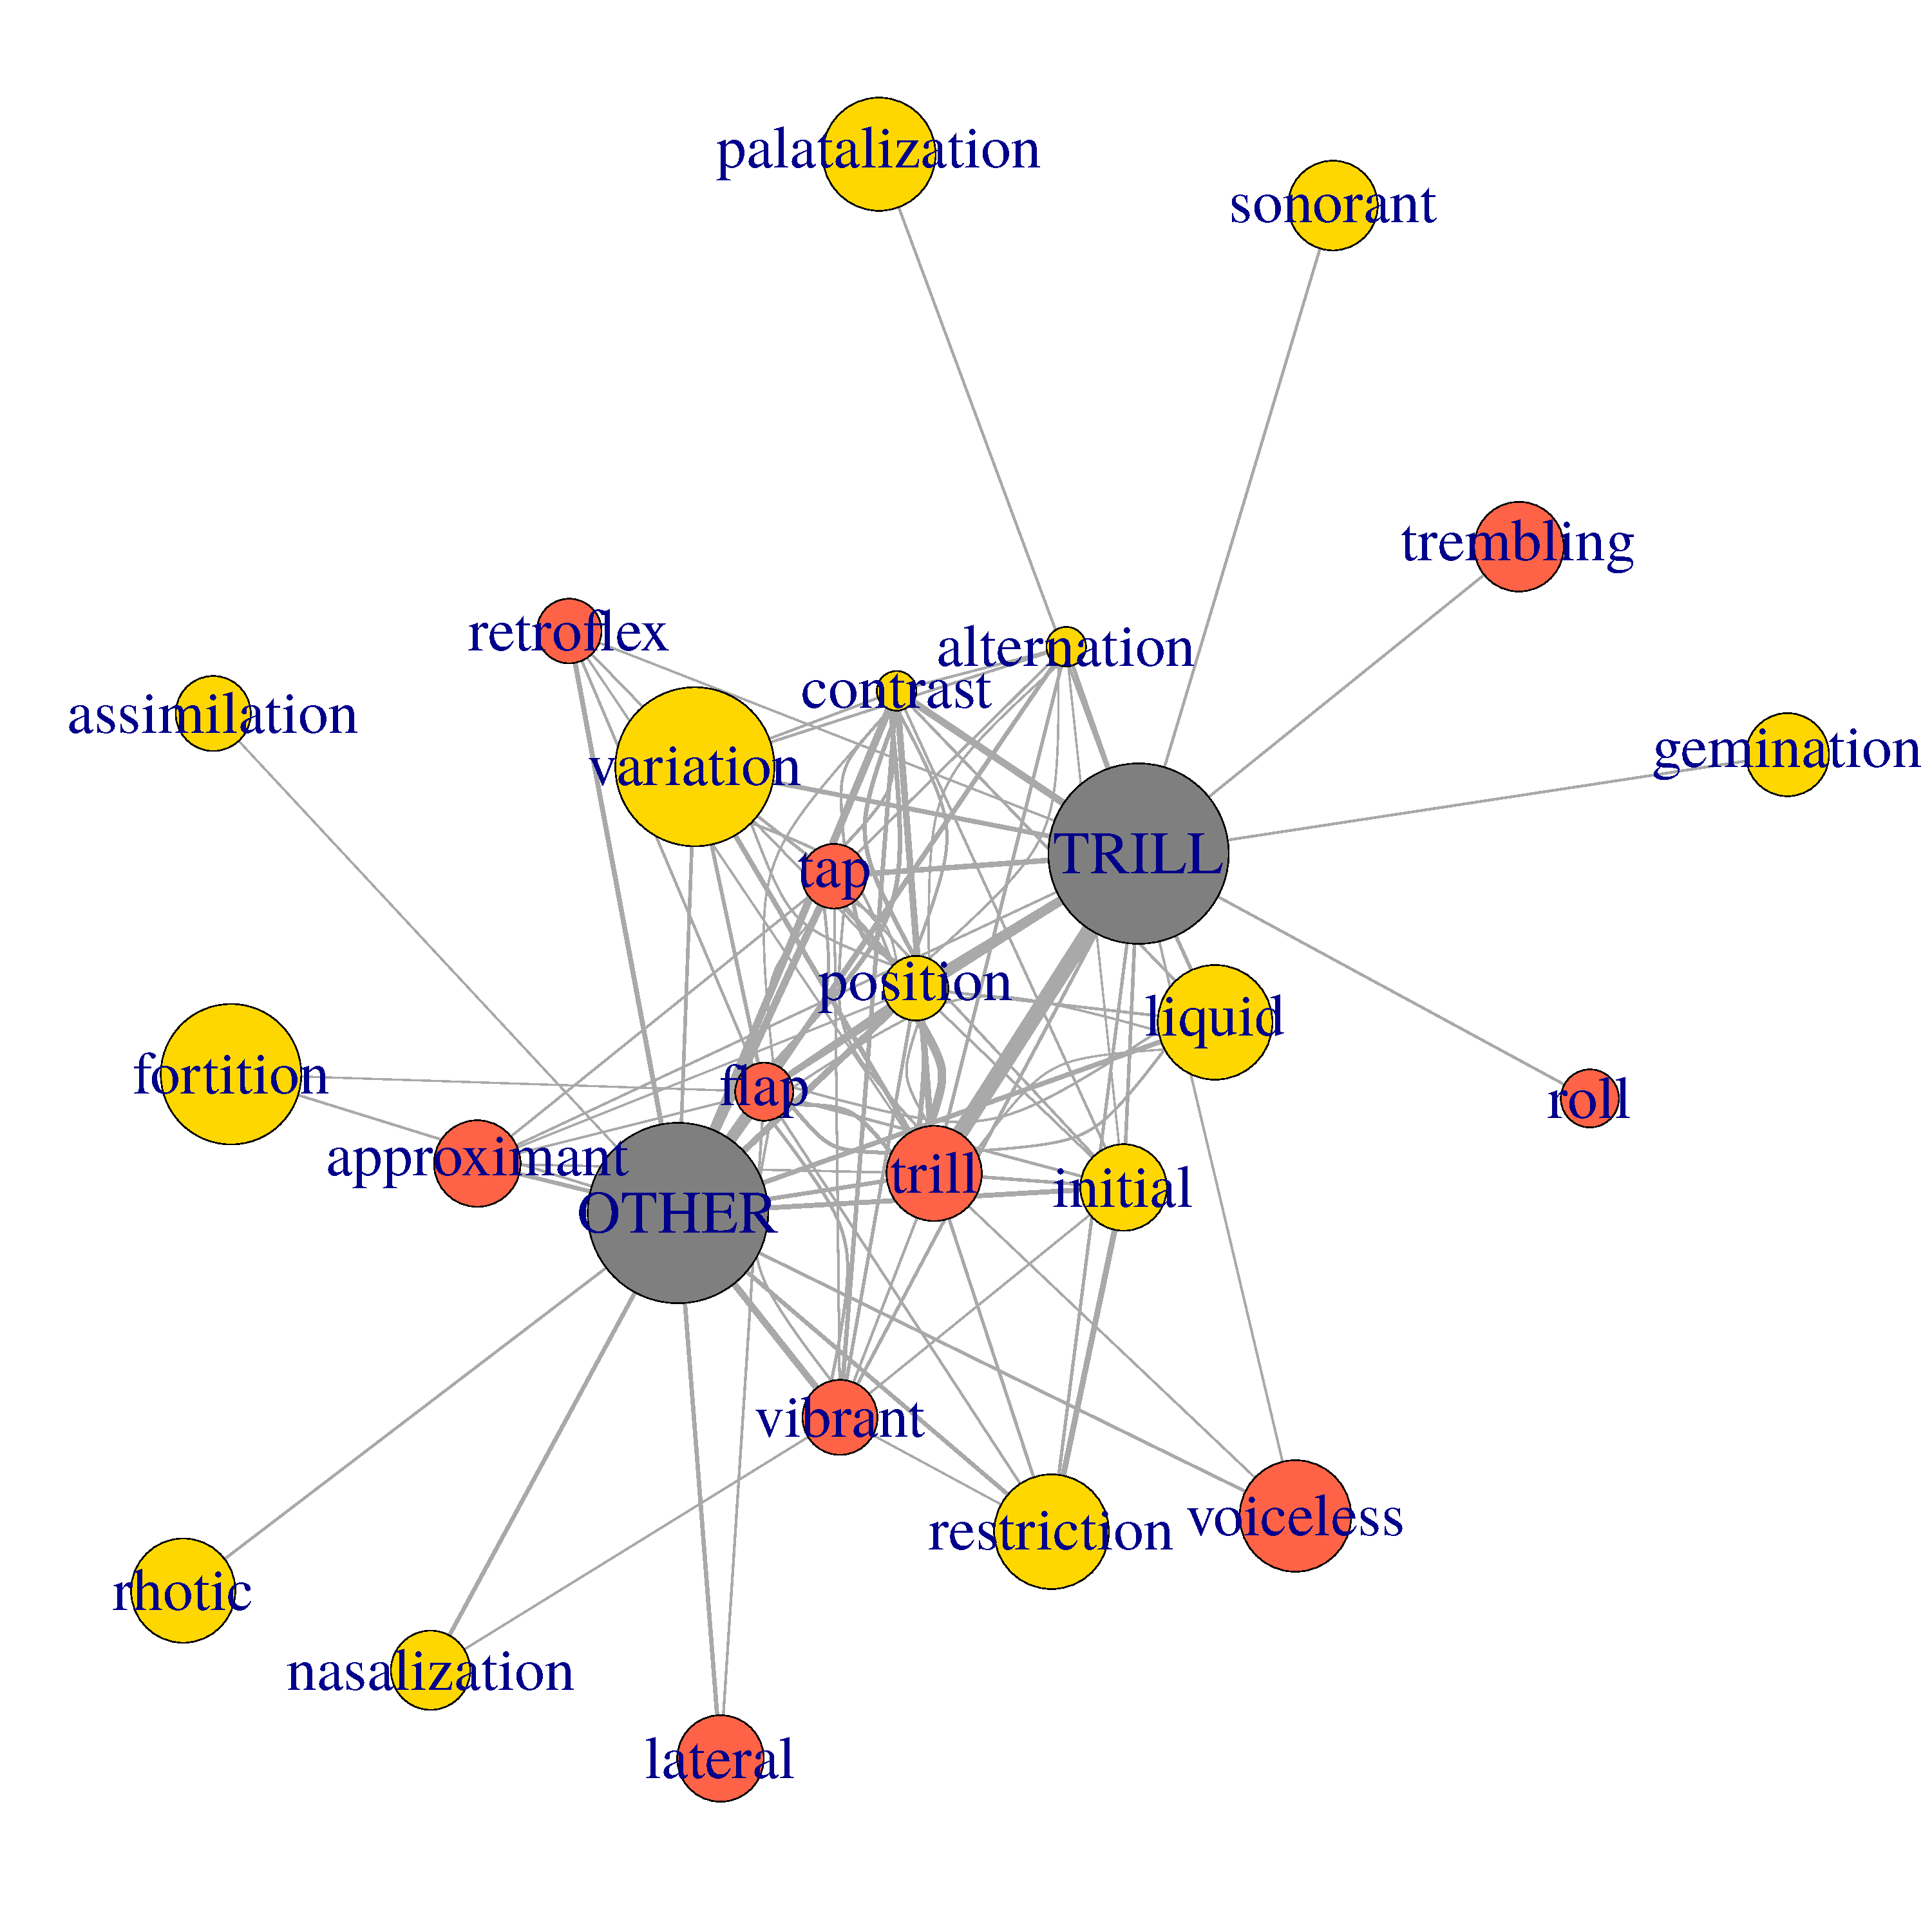
\includegraphics[width=1\linewidth]{substance/images/graph_results}
	\caption[Graphe des associations des différents concepts de phonétique et de phonologie à \textg{\textsc{trill}} et à \textg{\textsc{other}}]{Graphe des associations des différents concepts de phonétique et de phonologie de grammaires décrivant des langues possédant un /r/ trillé \textg{\textsc{trill}} ou un autre segment rhotique \textg{\textsc{other}}. Seuls les concepts qui sont présents plus de dix fois dans les grammaires sont représentés dans ce graphe. Les cercles jaunes correspondent à des concepts de phonologie, alors que ceux en rouge correspondent à des concepts de phonétique. La taille des cercles jaunes et rouges correspond à la fréquence des concepts, et l'épaisseur des liens, à la fréquence de l'association entre le concept et \textg{\textsc{trill}} ou \textg{\textsc{other}}. Les différentes épaisseurs des liens et tailles des cercles ont été normalisées. Le graphe est obtenu grâce au package \texttt{igraph} sur R \parencite{csardiIgraphSoftwarePackage2006}.}
	\label{fig:graphresults}
\end{figure}

Du fait du grand nombre de concepts annotés, nous avons choisi de représenter les différences entre les deux types de grammaires par un graphe où chaque nœud représente un concept. Ce graphe permet de mettre en évidence le manque de frontière entre ce qui est un trill et ce qui est une autre rhotique. Les concepts que nous avons pris en compte peuvent se retrouver autant dans des grammaires avec des trills que dans des grammaires avec les autres rhotiques.\\

La caractérisation des grammaires avec un si grand nombre de concepts étant peu aisée, nous souhaitions savoir si les termes de \textg{trill}, \textg{tap} et \textg{flap} étaient des bons prédicteurs de la possession d'une rhotique trillée dans la langue (selon nos données recodées issues de la réplication présentée dans le chapitre précédent).
Pour analyser nos données, nous avons élaboré plusieurs modèles linéaires généralisés à effets mixtes grâce au package \texttt{lme4} (\texttt{version 1.1-30}) et la fonction \texttt{glmer} \parencite{batesFittingLinearMixedeffects2015} sous R. Les différents modèles possédaient comme prédicteurs fixes les termes \textg{trill}, \textg{flap} et \textg{tap}. Nous avons contrôlé pour les familles de langues et les aires géographiques.\\

Les résultats d'un modèle qui prend en compte les trois termes indiquent que pour prédire la présence du \textg{trill} dans une langue, il y a un effet très significatif ($p < .001$) de ces trois termes. Cependant, en réalisant des modèles qui prennent chacun en compte un terme, le meilleur modèle (sur la base de sélection de modèle par critère AIC) était celui qui prédisait la présence du \textg{trill} dans une langue par le terme \textg{trill}. Autrement dit, la mention du terme \textg{trill} dans une grammaire est un prédicteur suffisant pour savoir si une langue doit être interprétée comme possédant un trill ou non.


%Nous avons de plus ajouté des informations complémentaires qui ne demandait pas trop d'effort de récupération.
%Nous avons pris en compte les fréquences des <r> à partir des dictionnaires inclus dans CLICS (Rzymski et al. 2019) avec comme hypothèse sous-jacente que les variétés avec un r fréquent serait plus décrite comme un trill, car avec le nombre d'occurence croissant, la probabilité de trillé pourrait se voir augmenter.
%Nous avons comparé cette fréquence avec celle des <l>, pour vérifier les fréquences des trill était différente de la même manière de celle des taps avec les latérales.
%L'intégration de données issus de dictionnaire nous a permis de voir si la présence de la rhotique en position initiale de mot n'était 
%Segment list
%IPA chart

%Consonants (Pulmonic)pas un facteur favorisant sa production comme un trill, et donc sa description comme un /r/ trillé, en sachant que les rhotiques ont tendance à éviter les position initiale de mot (Word-Initial Rhotic Avoidance) \parencite{labrunePhonologyJapanesePhonology2012}, ce qui aurait pu s'expliquer par la complexité de l'articulation du trill.

%Nous avons aussi intégré des informatios sur les patrons phonotactiques de chaque langue à partir d'une version archivée de World Phonotactitcs Database (WPD), dans le but de voir si la complexité syllabique était en relation avec les tap/flap \parencite{easterdayHighlyComplexSyllable2019} $\to$ A SUPPRIMER (problème de légalité)

%\subsection{Résultats}





%Modèle qui prédit revision en fonction:
%de trill : significatif
%262.0    278.2 
%de flap : significatif
%369.2    385.3 
%tap pas signicatif
%391.5    407.7 

%Et modèle :

%Bien que préliminaires les résultats que nous obtenons échouent à mettre en avant des différences entre \textsc{trill} et \textsc{other} dans les langues du monde en prenant comme prédicteurs les mots-clefs relevant de la phonologie.
%La significativité des résultats pour tout ce qui était facteur phonologique ($ \sim$ p<.05) était dépendante de si on contrôlait pour les macro-régions.


\subsection{Exemples de processus phonologiques associés aux rhotiques}

La visualisation des données est intéressante pour proposer des analyses exploratoires. Dans cette dernière section, nous souhaitons explorer trois exemples en relation avec la représentation du trill. D'après les données explorées (non présentées ici), nous avons remarqué que certains des concepts que nous avions annotés étaient plus associés à certaines régions du monde. À titre entièrement exploratoire, nous donnons l'exemple de la \textg{palatalisation} et de la \textg{nasalisation}. Dans notre perspective de typologie du trill, et de recherche de langues où la rhotique est réalisée comme un trill, nous explorons aussi les contrastes de longueur, dont certains étaient codés comme \textg{gémination} dans nos données.\\

Les trois exemples que nous donnons servent à mettre en avant que des inférences sur la réalisation des rhotiques dans certains cas restent possibles malgré le bruit dû aux différentes raisons mentionnées dans ce chapitre. Pour ces exemples, nous utiliserons, en parallèle des données de notre corpus, la base de données phonémiques PHOIBLE \parencite{phoible}. PHOIBLE, pour \textit{Phonetics information base and lexicon}, est définie comme \textg{online repository of cross-linguistic phonological segment inventory data that contains additional linguistic and non-linguistic information about languages} \parencite[171]{moranPhoneticsInformationBase2012}. La base de données comporte plus de 2000 langues pour plus de 3000 inventaires phonémiques. Certaines langues peuvent avoir plusieurs inventaires phonémiques. Les inventaires proviennent dans certains cas d'autres bases de données comme Stanford Phonology Archive (SPA, \cite{spa1979}) UCLA Segment Inventory Database (UPSID, \cite{maddiesonPatternsSounds1984,maddiesonprecoda1990}), South american phonological inventory database (SAPHON, \cite{saphon}), ou encore la base de données des Eurasian phonological inventories \parencite{nikolaev_etal2015}. Dans d'autres cas, il s'agit d'extractions d'inventaires à partir des sources secondaires (comme pour \cite{moran_etal2014}). PHOIBLE compile énormément de données dans lesquelles la représentation des rhotiques peut varier, ce que nous mettrons en évidence grâce à nos exemples.\\
%nous inte
%Des différents concepts que nous avons codées tous ne sont pas présents dans toutes les aires géographiques. Cela est en parti dû à notre échantillon de langues.
%Les termes de \textg{palatalisation} et de \textg{nasalisation} sont associés à la description des rhotiques dans certaines régions du monde et pas dans d'autres. Nous avons choisi d'illustrer la difficulté de la caractérisation des rhotiques avec ces deux processus.
%\paragraph{Exemple : Latéral}


\subsubsection{Exemple n°1 : Rhotiques et palatalisation}

Nous avons trouvé le terme de \textg{palatalisation} uniquement dans les grammaires d'Eurasie et d'Amérique du Sud.
Cependant, si on se réfère à PHOIBLE, la palatalisation des rhotiques n'est pas seulement présente sur ces deux macro-aires. En effet, on peut rencontrer de la palatalisation des rhotiques en Afrique, en Amérique du Nord et en Australie.
Le manque de données en Afrique dans notre échantillon (\autoref{fig:rhotiquespalatalization}) peut s'expliquer par le choix de garder les mêmes données que \textcite{winterTrilledAssociatedRoughness2022} où l'Afrique était déjà sous-représentée.\\

La question reste de savoir pourquoi le terme de \textg{palatalisation} semble ressortir (\autoref{fig:graphresults}) comme plus associé avec les langues où on retrouve un trill qu'avec les langues avec une autre rhotique ?\\

La littérature sur la palatalisation des rhotiques se concentre généralement sur le russe et sur les langues slaves \parencite{proctorGesturalCharacterizationPhonological2009,kavitskayaTrillsPalatalizationConsequences2009,kochetovIncompatibilityTrillingPalatalization2015}. \textcite{kochetovIncompatibilityTrillingPalatalization2015}, sur la base d'une étude exploratoire, montrent que la palatalisation produit un environnement défavorable pour la réalisation du trill (p. 2190). \textcite{kavitskayaTrillsPalatalizationConsequences2009} explique que ce sont des contraintes physiques conflictuelles au niveau du dos de la langue qui permettent d'expliquer la dépalatalisation dans certaines langues slaves. \textcite{dickey1997phonology,hallTypologicalGeneralizationsConcerning2000} s'intéressent à la palatalisation d'un point de vue typologique mais ne font pas de distinction entre trill et non trill, il s'agit de rhotiques dans les deux cas. \textcite{hallTypologicalGeneralizationsConcerning2000}\footnote{Nous noterons que \citeauthor{hallTypologicalGeneralizationsConcerning2000} mentionne que \textg{[s]ignificantly, many traditional grammarians are often not aware of the term \textg{approximant}}. \parencite[8]{hallTypologicalGeneralizationsConcerning2000}, justifiant \textit{a posteriori} l'intérêt modéré que nous avons pour les approximantes.} met en avant que les rhotiques palatalisées ne sont pas fréquentes, et les considère comme  plus marquées que d'autres types de segments palatalisés.\\ %L'auteur considère les rhotiques palatalisés comme plus marquées (ici plus un segment marqué, moins il est fréquent) par rapport à d'autres segments palatalisés. Ses travaux sur des langues indo-européennes et non-indo-europénnes, avec des données provenant principalement de UPSID, permettent de faire des prédictions sur les langues. L'auteur déclare que si une langue à une rhotique palatalisé, alors la même langue aura au moins un segment non-rhotique palatalisé. 

\begin{figure}
	\centering
	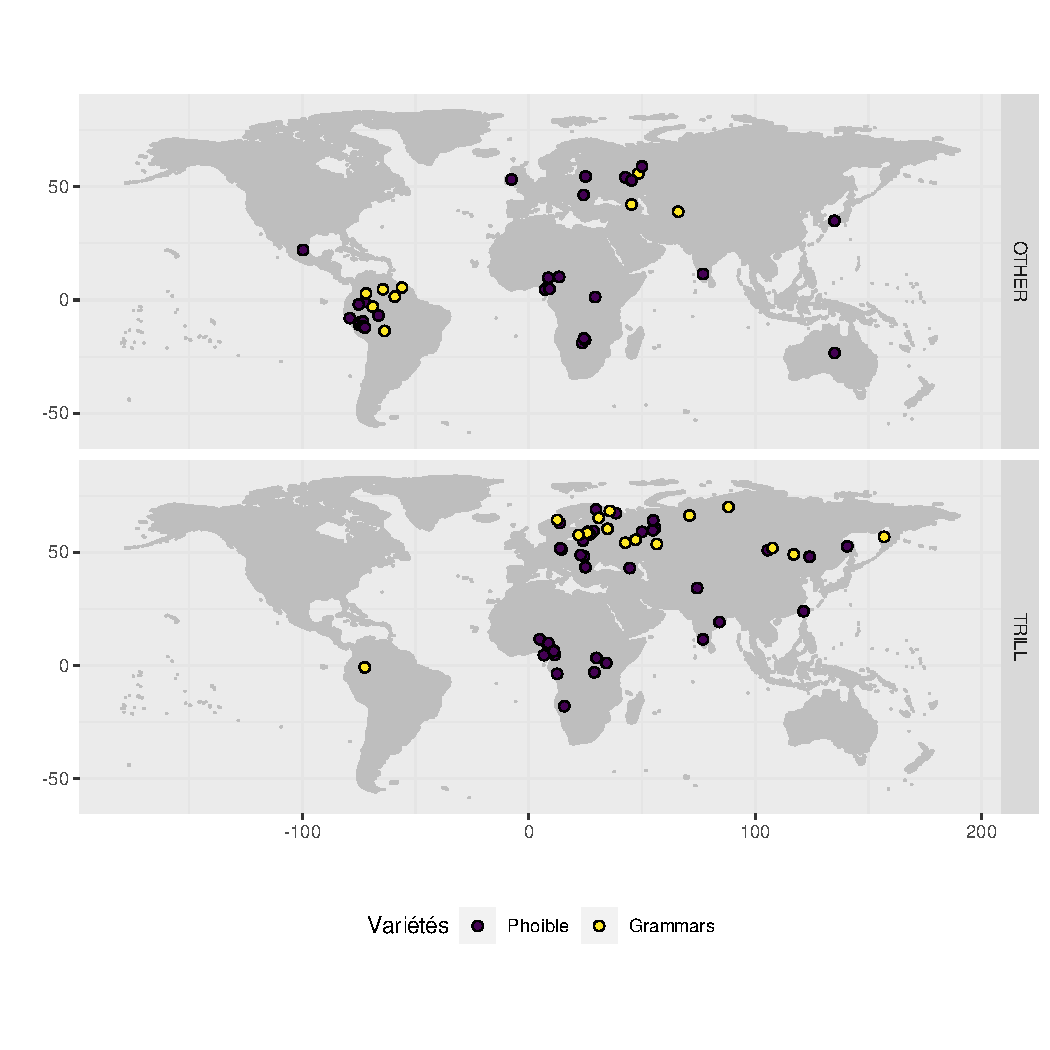
\includegraphics[width=1\linewidth,
	trim={0 1.65cm 0 1.65cm}, clip]{substance/images/rhotiques_palatalization}
	\caption[Distribution dans les langues du monde des rhotiques palatalisées]{Distribution dans les langues du monde des rhotiques palatalisées. Dans PHOIBLE seuls les symboles suivants sont pris en compte: ɽ, ɾ et ɻ pour les langues classifiées comme \textsc{other} (en haut) et r pour celles classifiées comme \textsc{trill} (en bas). Nous n'avons pas exclu les langues indo-européennes de PHOIBLE pour avoir un meilleur aperçu typologique.}
	\label{fig:rhotiquespalatalization}
\end{figure}

En s'interéssant aux données de PHOIBLE, on retrouve dans 25 langues non-indo-européennes pour 29 inventaires un segment représenté par /rʲ/ (et ses dérivés non-voisés ou rétractés). Des 29 inventaires, seulement huit ont des allophones reportés et il s'agit systématiquement du [rʲ].
Pour les autres segments \textg{simil-r} (\textit{ɽ}, \textit{ɾ}, \textit{ɻ}~~), PHOIBLE comprend 22 langues pour 24 inventaires.\\


Pour les trills palatalisés, on a les familles de langues suivantes :

\begin{exe}
	\ex \begin{xlist}
	\ex La famille linguistique ouralienne \glotto{ural1272} (16 inventaires)
	\ex La famille linguistique austronésienne \glotto{aust1307} (1 inventaire)
	\ex La famille linguistique austroasiatique \glotto{aust1305} (1 inventaire)
	\ex La famille linguistique atlantico-congolaise \glotto{atla1278} (6 inventaires)
	\ex La famille linguistique mongolique  \glotto{mong1329} (3 inventaires)
	\ex La famille linguistique dravidienne \glotto{drav1251} (2 inventaires)
	\end{xlist}
\end{exe}

Les familles où les autres segments \textg{simil-r} palatalisés se retrouvent sont :

\begin{exe}
		\ex \begin{xlist}
	%\item La famille linguistique dravidienne \glotto{drav1251} (4 inventaires)
	\ex La famille linguistique atlantico-congolaise \glotto{atla1278} (8 inventaires)
	\ex La famille linguistique ouralienne \glotto{ural1272} (3 inventaires)
	%\item La famille linguistique japonique \glotto{japo1237} (1 inventaire)
	%\item La famille linguistique chamito-sémitique \glotto{afro1255} (1 inventaire)
	%\item La famille linguistique ijoïde \glotto{ijoi1239} (1 inventaire)
	\ex La famille linguistique oto-mangue \glotto{otom1299} (1 inventaire)
	\ex La famille linguistique soudanique centrale \glotto{cent2225} (1 inventaire)
	%\item La famille linguistique austroasiatique \glotto{aust1305} (1 inventaire)
	\ex La famille linguistique arawakienne \glotto{araw1281} (7 inventaires)
	\ex La famille linguistique arawane \glotto{araw1282} (1 inventaire)
	\ex La famille linguistique borane \glotto{bora1262} (1 inventaire)
	\ex La famille linguistique zaparoane \glotto{zapa1251} (1 inventaire)
	%\item La famille linguistique pama-nyungan \glotto{pama1250} (1 inventaire)
	%\item La famille linguistique mongolique \glotto{mong1329} (1 inventaire)
	\ex La famille linguistique turcique \glotto{turk1311} (1 inventaire)
	\end{xlist}
\end{exe}

Dans les langues atlantico-congolaises et ouraliennes on trouve des trills palatalisés mais aussi d'autres segments \textg{simil-r} palatalisés.

Nous essayons d'expliquer la différence entre les langues atlantico-congolaises décrites avec un trill (n=6) et celles décrites avec un autre segment rhotique (n=7). Le rigwe (discuté plus bas), quant à lui, est compté deux fois car il possède un contraste entre /r/ et /ɾ/ selon PHOIBLE.

\begin{exe}
	\ex \begin{xlist}		
	\ex \href{https://phoible.org/inventories/view/1365}{Nyanga} \glotto{kuny1238} : on trouve un /r/, un /rʲ/ et un /rʷ/. La seule source mentionnée dans PHOIBLE est \textcite{kadimaEsquissePhonologiqueMorphologique1965}. Le système de transcription orthographique est celui de l'Alphabet International Africain (p. 59), et le système de transcription phonétique est celui de l'API. Page 62, on constate la mention de \textg{vibré} pour le /r/. Page 63, la mention \textg{combinaison de consonne avec semi-voyelle} est associée à \textg{ry} et à \textg{rw}. Page 64 se trouve la transcription phonétique [mbúr$^\textrm{\tiny i}$a].
	
	\begin{displayquote}
		\item \textbf{r} shall stand for the rolled lingual (tongue-tip) r of Scottish pronunciation or for the fricative r of Southern English.\footnote{Il existe une traduction en français : \textg{\textbf{r} s'emploie soit pour la roulée linguale telle qu'elle se prononce dans la campagne française et en Écosse, soit pour le r fricatif de 1'Anglais méridional.}. Dans le tableau des consonnes de l'ouvrage en anglais, il est inscrit \textg{rolled and flapped} alors que dans la traduction française il est uniquement inscrit \textg{Roulées} (p. 15)}\\ \parencite[9]{internationalafricaninstitutePracticalOrthographyAfrican1930}.
	\end{displayquote}

	\ex \href{https://phoible.org/inventories/view/1367}{Orusyan} \glotto{masa1299} : on trouve un /r/, un /rʲ/ et un /rʷ/. Nous n'avons pas trouvé la référence associée à l'inventaire : Huntingford, G. W. B. 1965. The Orusyan Language of Uganda.
	
	\ex \href{https://phoible.org/inventories/view/1503}{Kwambi} \glotto{kwam1251} : on trouve un /r/ et un /rʲ/. Nous n'avons pas trouvé la référence associée à l'inventaire : Baucom, Kenneth. 1972. The Wambo languages of South West Africa and Angola.
	
	\ex \href{https://phoible.org/inventories/view/1535}{West Kainji} \glotto{kagf1238} : on trouve un /r/, un /rʲ/ et un /rʷ/. Dans la référence associée, le terme de \textg{trill} est utilisé par  \textcite{smithNounClassSystem2007} dans le tableau des consonnes (p. 12).
	
	\ex \href{https://phoible.org/inventories/view/1537}{Rigwe} \glotto{irig1241} : on trouve un /r/, un /rʲ/ et un /rʷ/. À cela s'ajoutent aussi les phonèmes /ɾ/, /ɾʲ/ et /ɾʷ/. La source d'origine est \textcite{danielPhonologyRigweLanguage2008}.
	Page 21, les flaps et les trills sont décrits. Ainsi, le /ɾ/ est une flap alvéolaire avec une contrepartie labiale et palatale. Il existe des paires minimales entre /ɾ/ et /ɾʲ/, et /ɾ/ et /ɾʷ/. Le /ɾ/ contraste aussi avec le /r/ qui est décrit comme un trill alvéolaire qui possède aussi une contrepartie labiale et palatale.  /r/ contraste avec /rʲ/ dans un seul cas (rà vs. rʲâ; notons aussi le changement de ton). /rʲ/ est souvent substitué par /ɾʲ/. De plus /r/, contraste aussi avec /rʷ/ dans un seul mot.
	
	\ex \href{https://phoible.org/inventories/view/1599}{Mbe} \glotto{mbee1250} : on trouve un /r/, un /rʲ/ et un /rʷ/. Nous n'avons pas trouvé la référence associée à l'inventaire : Pohlig, James. 1981. The Mbe verb: A description of the verb system of Mbe, a language of Northern Cross River State, Nigeria. (unpublished).
	
	\ex Igbo \glotto{nucl1417} : on trouve plusieurs inventaires dans PHOIBLE. SPA reporte \href{https://phoible.org/inventories/view/143}{/ɾ/ et /ɾʲ/}, UPSID reporte \href{https://phoible.org/inventories/view/365}{/ɾ̪ʲ|ɾʲ/ et /ɾ̪ʲ|ɾʲ/}, Alphabets of Africa reporte \href{https://phoible.org/inventories/view/732}{/r/} et l'extraction de \textcite{moran_etal2014} fait état de \href{https://phoible.org/inventories/view/2192}{/ɹ/}. Le /ɹ/ dans ce dernier inventaire provient de l'Illustration of the IPA du igbo \parencite{ikekeonwuIgbo1991}.
	
	\ex \href{https://phoible.org/inventories/view/852}{Fwe} \glotto{fwee1238} : On trouve /ɻ/, /ɻʲ/, /ɻʷ/ et /rʷ/. Nous n'avons pas trouvé la référence associée à l'inventaire : Baumbach, Erdmann J.M. 1997. Languages of the Eastern Caprivi. Pour cela nous avons consulté \textcite{gunninkGrammarFweBantu2018} (pp. 21-22) qui mentionne \textg{alveolar tap /r/ is phonemic} et que lorsque /r/ est suivi d'une approximante palatale, il est réalisé comme un [l].
	
	\ex \href{https://phoible.org/inventories/view/853}{Yeyi} \glotto{yeyi1239} : On retrouve /r/, /rʷ/, /ɻ/ et /ɻʲ/. Nous n'avons pas trouvé la référence associée à l'inventaire : Baumbach, Erdmann J.M. 1997. Languages of the Eastern Caprivi.
	
	\ex \href{https://phoible.org/inventories/view/1202}{Subiya} \glotto{subi1246} : On retrouve /ɻ/, /ɻʲ/ et /ɻʷ/. Nous n'avons pas trouvé la référence associée à l'inventaire : Baumbach, Erdmann J.M. 1997. Languages of the Eastern Caprivi.
	
	\ex \href{https://phoible.org/inventories/view/1203}{Totela} \glotto{tote1238} : On retrouve /ɻ/, /ɻʲ/ et /ɻʷ/. Nous n'avons pas trouvé la référence associée à l'inventaire : Baumbach, Erdmann J.M. 1997. Languages of the Eastern Caprivi.
	
	\ex \href{https://phoible.org/inventories/view/1533}{Iten} \glotto{eten1239} : On retrouve /ɾ/, /ɾʲ/, /ɾʷ/ et /ɾʷʲ/. Dans la source \textcite{blenchItenConsonantAlternation2010} on retrouve la mention de \textg{Tap} associée avec le r (p. 3). Il est écrit que ry est une consonne labialisée, mais il doit s'agir d'une erreur, de même pour rw qui est palatalisé (le plus probable est qu'il s'agisse d'une erreur d'inversion entre les deux termes). ryw est une consonne palatale-labiale.
	\end{xlist}
\end{exe}


La famille atlantico-congolaise est grande. En effet, il existe plusieurs sous-branches dans son arbre phylogénique. Toutes les langues que nous avons prises en exemple sont des langues issues de la branche bénoué-congolaise. Les langues que nous avons utilisées appartiennent aux langues bantoues, aux langues kainji, aux langues du plateau nigérian et aux langues igboïdes. L'exemple de la palatalisation dans ces différentes langues, qui pourtant appartiennent à la même branche, illustre les différences de représentations entre les bases de données. De plus, nous soulignons la curiosité qu'est la langue rigwe. Si le rapport des différents segments est exacte, alors il s'agit d'une langue typologiquement intéressante pour les rhotiques. Cependant, nous n'avons pas trouvé, pour vérifier, des références autres que l'ouvrage non publié de \textcite{danielPhonologyRigweLanguage2008} que nous citons.\\

Bien que le trill défavorise la palatalisation, certaines grammaires mentionnent les deux termes. Les langues avec une rhotique palatalisée possèdent aussi une rhotique non palatalisée. Lorsque la rhotique non palatalisée est représentée par un \textit{r}, alors sa contrepartie palatalisée le sera avec un \textit{r}, même si son articulation n'est pas trillée. Plus de langues décrites comme possédant un trill implique donc plus de langues décrites comme possédant un trill palatalisé.


%dépendant de comment est représenté la contrepartie non palatalisé, donc du biais initial en faveur du trill.


\subsubsection{Exemple n°2 : Rhotiques et nasalisation}

Après nous être intéressé à la \textg{palatalisation}, nous analysons la \textg{nasalisation}. C'est un terme que nous retrouvons dans les grammaires d'Amérique du Sud et d'Afrique. Il s'agit dans de nombreux cas d'un terme qui fait référence à l'harmonie nasale qu'on retrouve dans les langues des deux macro-aires géographiques \parencite{pengNasalHarmonyThree2000,clementsIkwereNasalHarmony2003,clementsNasalHarmonyIkwere2005}.\\

\begin{figure}
	\centering
	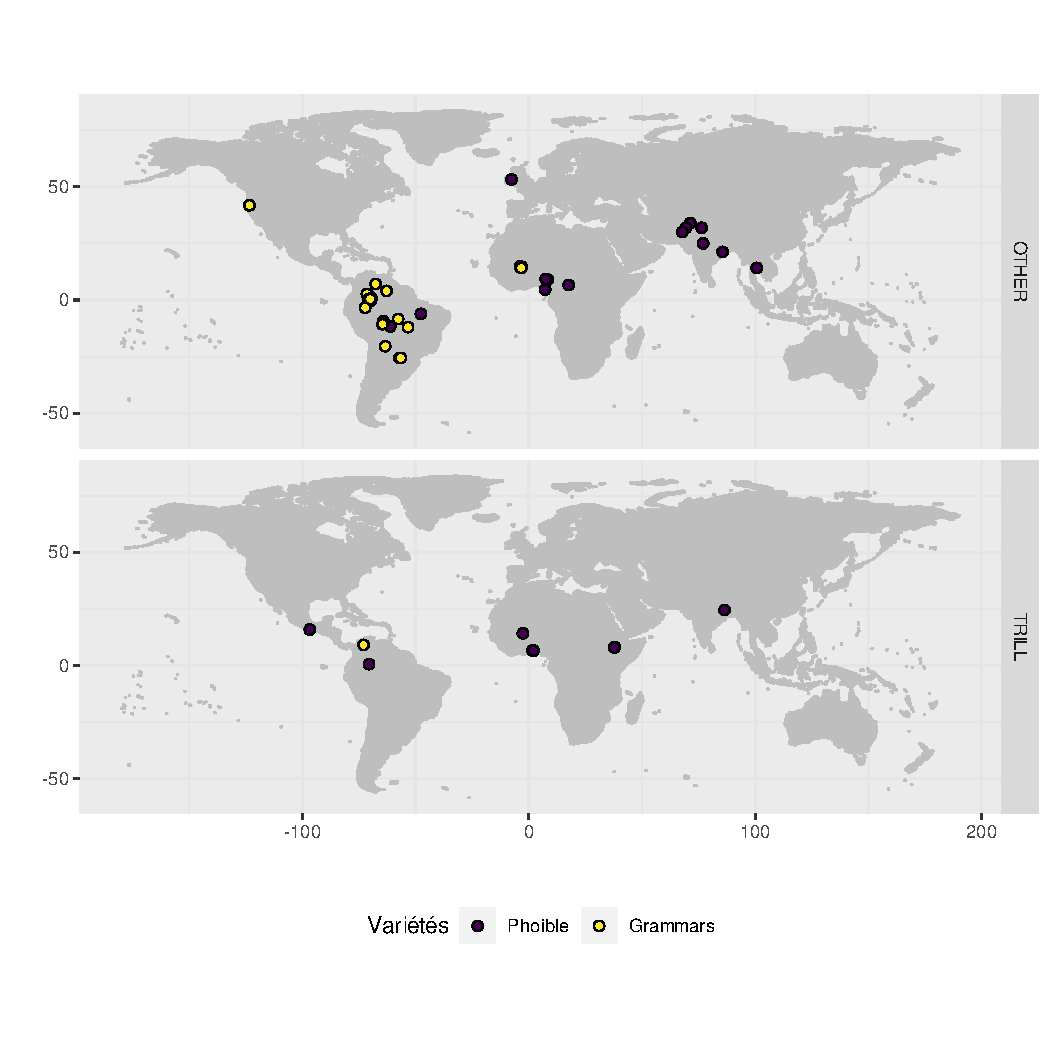
\includegraphics[width=1\linewidth,
	trim={0 1.65cm 0 1.65cm}, clip]{substance/images/rhotiques_nasalization}
	\caption[Distribution dans les langues du monde des rhotiques nasalisées]{Distribution dans les langues du monde des rhotiques nasalisées. Dans PHOIBLE seuls les symboles suivants sont pris en compte: ɽ, ɾ et ɻ pour les langues classifiées comme \textsc{other} (en haut) et r pour celles classifiées comme \textsc{trill} (en bas). Nous n'avons pas exclu les langues indo-européennes de PHOIBLE pour avoir un meilleur aperçu typologique.}
	\label{fig:rhotiquesnasalization}
\end{figure}


Contrairement à la  \textg{palatalisation}, le \textsc{trill} n'apparaît pas avec le terme \textg{nasalisation}. Dans nos données, il existe une exception, celle de la langue barí \glotto{bari1297}. La rhotique présente dans PHOIBLE est \href{https://phoible.org/inventories/view/1892}{/r/}. Notre recodage a abouti à dire que la langue possédait un /r/ trillé. La nasalisation est présente dans \textcite{mogollonperezFonologiaLenguaBari2000}. Néanmoins, il faut prendre en compte les commentaires de \citeauthor{mogollonperezFonologiaLenguaBari2000} pour se rendre compte que ce n'est pas le [r] qui est nasalisé. L'analyse phonologique de l'autrice oppose un /r/ à un /n/ (p. 719). Ce phonème /n/ possède quatre allophones dont un tap et un tap nasalisé [ɾ̃] apparaissant entre deux voyelles nasales. Le /r/ se réalisant comme une \textg{vibrante multiple} ne se trouve pas entre deux voyelles nasales.\\

Nous mettons en perspective nos données avec celles de PHOIBLE. En ce qui concerne les nasales rhotiques dans PHOIBLE, nous avons recherché les segments qui pourraient correspondre à [r̃]  mais aussi à [ɾ̃] (nous n'illustrons pas le segment suivant : [ɽ̃] qui est inclus dans la \autoref{fig:rhotiquesnasalization}) dans les allophones des rhotiques donnés par la base de données. Nous avons obtenu les cas intéressants suivants :

\begin{exe}
	\ex \begin{xlist}

	\ex \href{https://phoible.org/inventories/view/7}{Kurukh} \glotto{kuru1302} : on a avec les données de PHOIBLE l'allophone r̠̃. Il s'agit d'une langue appartenant à la famille dravidienne. On trouve sur PHOIBLE à partir de SPA trois sources datant de 1924, 1964 et de 1972. L'inventaire reporte un /r̠/ dont un des trois allophones est [r̠̃]. On retrouve aussi dans la langue un /r/ et un /rː/. UPSID ne mentionne que \href{https://phoible.org/inventories/view/429}{/r̪|r/ et /r̠/} sans rhotique nasalisée en allophone. \textcite[36]{kobayashiKuruxLanguageGrammar2017} mentionne que /ɽ/ (= /r̠/) peut être réalisé comme un [ɳ] sur la base de Grignard (1924) qui était une des sources de SPA. Nous n'avons donc aucune raison de penser qu'il y ait un trill nasalisé dans la langue.
	
	\ex \href{https://phoible.org/inventories/view/1022}{Zapotec} \glotto{loxi1235} : on a, avec les données de PHOIBLE, l'allophone r̃. Il s'agit d'une langue appartenant à la famille otomanguean. L'interprétation est différente de celle du kurukh. En effet, \textcite{beamdeazconaCoatlanLoxichaZapotecGrammar2004} mentionne que la variété décrite comporte deux sons rhotiques : un [ɾ] et un [r̃] (p. 47). Cependant, il ne s'agit ici pas d'API mais d'un mélange entre plusieurs alphabets phonétiques, plusieurs traditions de transcriptions. Le fait de savoir que les segments adoptent une distribution similaire à celle de l'espagnol, à cause des emprunts à la langue avec le [r̃] en position initiale ou finale de syllabe, et qu'il n'y ait pas de mention de nasalisation, laisse à penser qu'il s'agit d'une rhotique avec deux allophones de longueurs différentes : un [ɾ] et un [r]. Nous n'avons donc aucune raison de penser qu'il y ait un trill nasalisé dans la langue.
	
	\ex \href{https://phoible.org/inventories/view/1040}{Tatuyo} \glotto{tatu1247} : on a, avec les données de PHOIBLE, l'allophone ɾ̃. Il s'agit d'une langue appartenant à la famille tucanoan. Le segment nasalisé est un allophone du /r/ qui possède aussi un [r] comme allophone et un [l]. Nous n'avons donc aucune raison de penser qu'il y a un trill nasalisé dans la langue.
	
	\ex \href{https://phoible.org/inventories/view/1279}{xwela} \glotto{xwel1235} : on a, avec les données de PHOIBLE, l'allophone r̃. Il s'agit d'une langue appartenant à la famille atlantico-congolaise. A priori, il y a dans la langue un [r] et un [r̃]. La source donnée est celle de \textcite{capoComparativePhonologyGbe1991}. Page 49, il est mentionné que le r̃ fait référence à un \textg{nasalised apical (post) alveolar trill} pour les dialectes Gbe. Le segment est toujours la deuxième consonne d'une attaque branchante en initiale de mot, où la première consonne est coronale. Les trois langues de cette liste ont la même référence.
	\ex \href{https://phoible.org/inventories/view/1280}{western xwla} \glotto{west2456} : on a, avec les données de PHOIBLE, l'allophone r̃. Il s'agit d'une langue appartenant à la famille atlantico-congolaise. La source de l'inventaire est la même que pour le xwela.
	\ex \href{https://phoible.org/inventories/view/1281}{kotafon} glotto{kota1272} : on a, avec les données de PHOIBLE, l'allophone r̃. Il s'agit d'une langue appartenant aux langues atlantico-congolaises. La source de l'inventaire est la même que pour le xwela.
	\ex \href{https://phoible.org/inventories/view/1282}{gbesi} \glotto{gbes1238} : on a, avec les données de PHOIBLE, l'allophone r̃. Il s'agit d'une langue appartenant à la famille atlantico-congolaise. La source de l'inventaire est la même que pour le xwela.
	\begin{itemize}
		\item \textcite{capoComparativePhonologyGbe1991} décrit le Eastern Gbe. Uniquement avec cette source, il faudrait conclure que les trills nasalisés existent dans les quatre langues mentionnées. Cependant, nous avons choisi de mettre en contraste cette source avec  \textcite{lotvenSoundSystemSketch2020} sur le Gen du Western Gbe. Parmi les liquides mentionnées par l'auteur (p. 8), on ne retrouve plus de trills nasalisés mais des [ɾ̃] et des [ɾ̃]. Nous ne pouvons pas, à ce stade, rejeter la possibilité de trill nasalisé, cependant nous n'y accordons que peu de crédibilité.
	\end{itemize}
	\ex \href{https://phoible.org/inventories/view/1442}{Jamsay, Dogon} \glotto{jams1239} : on a, avec les données de PHOIBLE, l'allophone r̃. Il s'agit d'une langue appartenant à la famille dogon. PHOIBLE mentionne trois segments rhotiques : /r/, /rː/ et /r̃/. La source donnée est \textcite[34]{heathGrammarJamsay2008}. On retrouve à la page 71 la mention de \textg{trill} en association avec <rr>. Le trill existe aussi dans les emprunts au \href{https://glottolog.org/resource/languoid/id/fula1264}{Fulfulde} de la famille Atlantique-Congo. Cela laisse l'interprétation libre au fait que le r n'est probablement pas réalisé comme un trill mais comme un tap/flap (aucun des deux termes n'est cependant mentionné dans la grammaire). De plus, il existe une règle de dérhotisation où /r$^{n}$/ devient un [n] avant un consonne ou en coda de mot (p. 69). Pour toutes ces raisons, nous n'avons aucune raison de penser qu'il y a un trill nasalisé dans la langue.
	
	\ex \href{https://phoible.org/inventories/view/1464}{Gyeto} \glotto{seba1251} : on a, avec les données de PHOIBLE, l'allophone r̃. Il s'agit d'une langue appartenant à la famille chamito-sémitique. On trouve dans PHOIBLE deux phonèmes /r/ et /r̃/. Nous n'avons pas trouvé la référence associée à l'inventaire : Hetzron, Robert. 1977. The Gunnan-Gurage Languages. Instituto Orientale di Napoli. Il s'agit de la même source pour les langues suivantes.

	\ex \href{https://phoible.org/inventories/view/1465}{Ennemor} \glotto{inor1238}, \href{https://phoible.org/inventories/view/1466}{Endegen} ou \href{https://phoible.org/inventories/view/1467}{Ener} : on a, avec les données de PHOIBLE, l'allophone r̃ pour les trois inventaires. Il s'agit de langues appartenant à la famille chamito-sémitique. PHOIBLE mentionne aussi deux phonèmes /r/ et /r̃/.
	\begin{itemize}
		\item Nous n'avons pas trouvé la référence de Hetzron (1977). Nous avons choisi à la place de nous baser sur la grammaire récente de \textcite{vollminGrammarGumerPhonologyMorphology2017}. L'auteur mentionne qu'il existe un seul phonème /r/ qui peut se réaliser comme un \textit{r} ou comme un \textit{n} lorsqu'il passe sous nasalisation. Aucune mention n'est faite dans la grammaire du terme \textg{trill}. Nous ne pouvons pas, à ce stade, rejeter la possibilité de trill nasalisé, cependant nous n'y accordons que peu de crédibilité.
	\end{itemize}
	\end{xlist}		
\end{exe}

%De plus, on retrouve de la variation dans les dénomination dans les descriptions intra-langues. Par exemple, pour les termes \textg{tap}-\textg{flap} (cf Section XXXX), certains auteurs vont plus parlé de trills alors que d'autres de taps. Cela peut-être dû à un effet de l'éducation des descripteurs, et que plus la personne a été formée proche de 2022, plus elle va avoir tendance à utiliser le terme \textg{tap} en dépit du terme \textg{flap}.

\textcite{soleAerodynamicCharacteristicsTrills2002} (p. 677-678) explique l'impossibilité de l'existence des trills nasalisés, qui étaient déjà mis en avant avec les données de UPSID \parencite{maddiesonPatternsSounds1984}. En effet, l'ouverture du velum pour les nasales fait chuter la pression intra-orale qui doit rester haute pour les trills. Une faible ouverture du velum peut néanmoins permettre de triller, cependant, le segment n'est pas perçu comme nasalisé si l'on se base sur les travaux de Maeda (1993)\footnote{Maeda, S. (1993) Acoustics of vowel nasalization and articulatory shifts in French nasal vowels. In Phonetics and phonology, Vol. 5: Nasals, nasalization, and the velum (M. K. Huffman \& R. A. Krakow, editors), pp. 147–167. San Diego, CA: Academic Press.}. Par sa nature différente du trill (c'est-à-dire sans contrainte aérodynamique aussi précise que pour le trill), le tap peut être nasalisé.\\

Le fait que le terme \textg{nasalisation} soit plus associé à des rhotiques qui ne sont pas réalisées comme des trills n'est donc pas un hasard, et illustre bien une différence aérodynamique entre les deux segments. 
Ainsi, nous pouvons dorénavant rejeter la possibilité de trill nasalisés dans des exemples pour lesquels c'était auparavant impossible.
Nous ne signalons pas à ce jour de trill nasalisé dans les langues du monde, mais uniquement des taps/flaps nasalisés.\\


Les exemples de \textg{nasalisation} et \textg{palatalisation} montrent que chercher ce qui relève du trill ou des autres rhotiques dans les grammaires n'est pas aisé, à cause de l'ambiguïté des représentations.
Mais alors comment chercher les trills ? Nous proposons un dernier exemple à travers les contrastes de longueurs dans les rhotiques.


\subsection{Exemple n°3 : Rhotiques et contraste de longueur}

Les exemples de \textg{palatalisation} et \textg{nasalisation} nous ont permis de mettre en avant les problèmes dus au travail avec des inventaires phonémiques. Pour autant, nous souhaitons montrer que bien que l'on ne puisse avoir aucune assurance qu'un trill est un trill, autre que par son étude acoustique et articulatoire, il est intéressant de se pencher sur les contrastes de longueur dans les rhotiques qui peuvent constituer une niche pour la subsistance du trill.\\

\begin{figure}
	\centering
	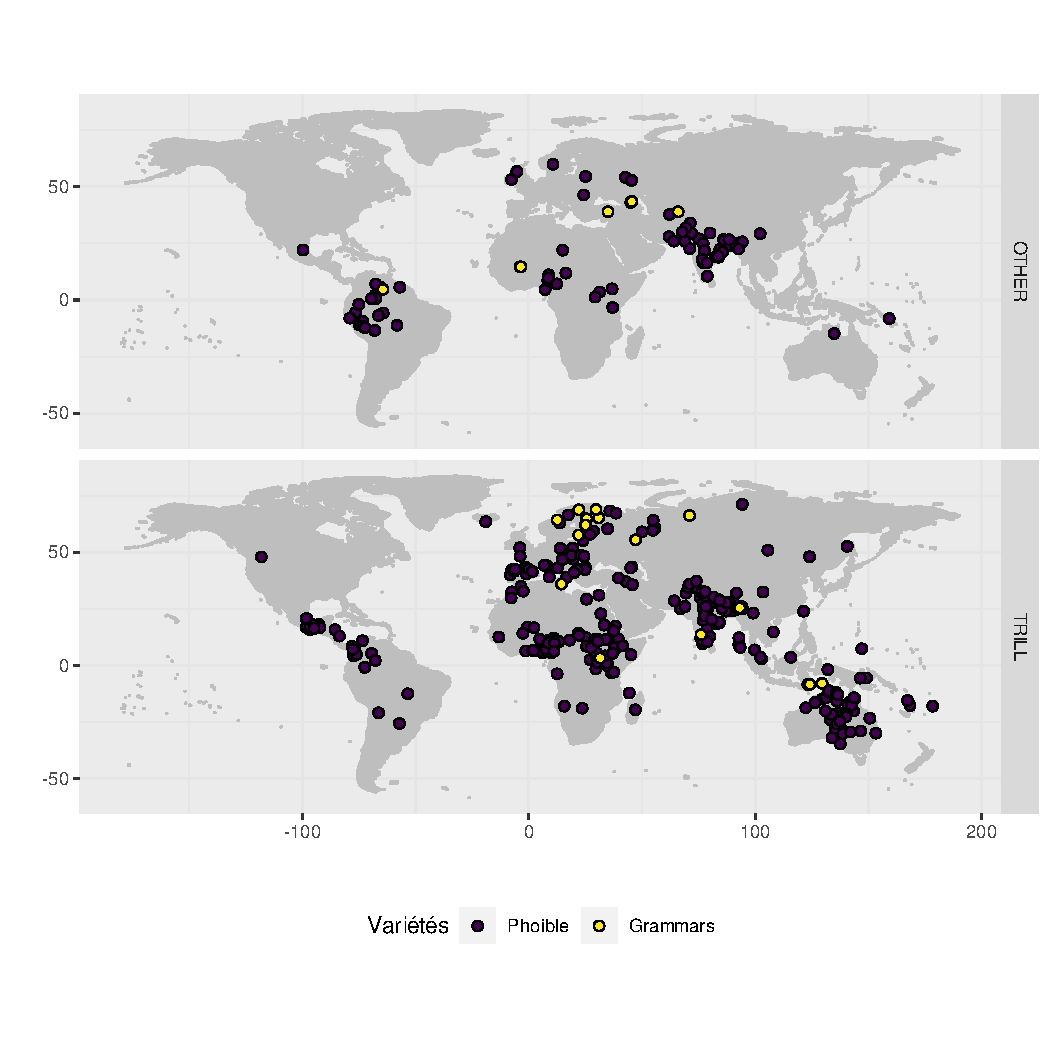
\includegraphics[width=1\linewidth,
	trim={0 1.65cm 0 1.65cm}, clip]{substance/images/rhotiques_gemination}
	\caption[Distribution dans les langues du monde des contrastes de longueur pour les rhotiques]{Distribution dans les langues du monde des contrastes de longueur pour les rhotiques. Dans PHOIBLE seuls les symboles suivants sont pris en compte: ɽ et ɾ pour les langues classifiées comme \textsc{other} (en haut) et r pour celles classifiées comme \textsc{trill} (en bas). Nous n'avons pas exclu les langues indo-européennes de PHOIBLE pour avoir un meilleur aperçu typologique.}
	\label{fig:rhotiquesgemination}
\end{figure}


À cette fin, nous avons choisi d'examiner le terme de \textg{gémination}, le seul des concepts que nous avions annoté qui permettait de mettre en avant un contraste de longueur. En effet, nous avions exclu toutes les langues qui devaient posséder deux rhotiques phonémiques dont l'une était un trill. Le contraste de longueur met en jeu deux rhotiques dont l'une est courte et l'autre est longue. L'hypothèse est que le contraste entre deux rhotiques permet une conservation du trill dans la langue, qui est généralement la rhotique longue, alors que la rhotique courte est un tap ou un flap.
La \textg{gémination} et les contrastes de longueur sont des phénomènes mesurables comme pour le arop-lokep \glotto{arop1243} qui oppose un trill simple et un trill géminé.
Au niveau des inventaires phonémiques, il n'y a généralement pas d'indication sur les contrastes de longueur. L'interprétation doit être faite à partir des symboles de l'API. La longueur est généralement indiquée par {\fontspec{Charis SIL}◌ː}, mais nous suggérons que ce n'est pas la seule manière.
Pour investiguer le contraste de longueur dans les rhotiques, nous illustrons à partir des données de PHOIBLE, en excluant les langues indo-européennes (sauf dans la \autoref{fig:rhotiquesgemination}), les inventaires de langues où :

\begin{exe}
	\ex \begin{xlist}
	\ex r contraste avec ɾ $\to$ 113 inventaires (auxquels il faudrait ajouter 32 inventaires pour les langues indo-européennes)
	\ex r contraste avec rː $\to$ 40 inventaires (auxquels il faudrait ajouter 7 inventaires pour les langues indo-européennes)
	\ex r contraste avec ɽ $\to$ 41 inventaires (auxquels il faudrait ajouter 69 inventaires pour les langues indo-européennes)
	\ex ɾ contraste avec ɽ $\to$ 41 inventaires (auxquels il faudrait ajouter 21 inventaires pour les langues indo-européennes)
	\ex ɾ contraste avec ɾː $\to$ \href{https://phoible.org/inventories/view/1525}{1 inventaire}
	\ex ɽ contraste avec ɽː $\to$ Non attesté
		\end{xlist}
\end{exe}

Nous avons fait le choix de ne pas inclure les approximantes /ɻ ɹ/ pour se concentrer uniquement sur les manières d'articulation \textg{trill} et \textg{tap/flap}.\\

Dans 18 inventaires (auxquels il faudrait ajouter 5 inventaires pour les langues indo-européennes), on a un un contraste de longueur mettant en jeu au moins plus de trois rhotiques. Il peut s'agir des triplets /r ɽ ɾ/ et /r  rː ɽ/.\\

Commençons à regarder les grammaires avec le contraste entre /ɾ/ et /ɾː/. L'utilisation du ɾː porte à confusion et est le résultat de l'interprétation des symboles faite par les contributeurs de PHOIBLE. Il s'agit d'une opposition entre un segment court et un segment long avec le segment court qui est réalisé comme un tap et le long comme un trill :

\begin{exe}
	\ex \href{https://phoible.org/inventories/view/1525}{Arbore} \glotto{arbo1245} : il s'agit d'une langue appartenant à la branche couchitique de la famille chamito-sémitique. Les données de PHOIBLE font mention d'un /ɾ/ et d'un /ɾː/. La phonologie de la langue a été décrite par \textcite{haywardArboreLanguageFirst1984}. Dans la source d'origine, on y retrouve un /r/ qui est réalisé phonétiquement comme un tap voisé alvéolaire (p. 54). Il existe un <rr> dans la langue qui est réalisé comme un [r] (p. 57). Il n'y a aucune mention de tap géminé.
\end{exe}

Pour ne pas avoir à travailler sur toutes les données de manière exhaustive, nous avons préféré échantillonner nos données. Nous avons obtenu un échantillon aléatoire de six langues pour le contraste entre /r/ et /rː/. Dans un seul cas sur six nous avons pu conclure qu'il existe vraiment deux segments natifs dont l'un est un trill. 

\begin{exe}
	\ex \begin{xlist}

	\ex \href{https://phoible.org/inventories/view/879}{Garadjari} \glotto{kara1476} : il s'agit d'une langue appartenant à la famille pama-nyungan. On trouve dans PHOIBLE /r/ qui contraste avec /rː/. Dans l'inventaire, le /rː/ est le seul segment géminé. Nous n'avons pas trouvé la référence associée à l'inventaire :  Sands, Anna Kristina. 1989. A Grammar of Garadjari, Western Australia.
	
	\ex \href{https://phoible.org/inventories/view/1418}{Krongo} \glotto{kron1241} : il s'agit d'une langue appartenant à la famille kadouglienne. On trouve dans PHOIBLE /r/ et /rː/. Dans \textcite{hallKadugliKrongo2004}, /r/ est une continuante (p. 59). Bien que \textg{[l]engthened forms of most consonants occur as geminates}, il n'est pas explicitement précisé si le /r/ peut être géminé et on ne retrouve de <rr> ou de <rː> dans aucun des exemples donnés par les auteurs.
	
	\ex \href{https://phoible.org/inventories/view/1419}{Kanga (Kanga)} \glotto{kang1288} : il s'agit d'une langue appartenant à la famille kadouglienne. On trouve /r/ et /rː/ dans PHOIBLE avec la même référence que pour le krongo \parencite{hallKadugliKrongo2004}.
	
	\ex \href{https://phoible.org/inventories/view/1442}{Jamsay, Dogon} \glotto{jams1239} : il s'agit d'une langue appartenant à la famille dogon. On trouve /r/ et /rː/ mais aussi /r̃/ dont nous avions parlé pour la nasalisation. \textcite{heathGrammarJamsay2008} mentionne qu'il ne connaît pas de radical contenant un rr géminé à l'exception de ceux qui sont empruntés au fulfulde (p. 71) et vraisemblablement réalisés comme des trills. Autrement, le /rr/ peut se retrouver en morphologie verbale où il est réalisé comme un [ll].
	
	\ex \href{https://phoible.org/inventories/view/1552}{Oromo, Eastern} \glotto{east2652} : il s'agit d'une langue appartenant à la branche couchitique de la famille chamito-sémitique. Dans PHOIBLE on retrouve /r/ et /rː/. Dans \textcite{owensGrammarHararOromo1985}, on trouve un /r/ qui peut être géminé (p. 22) sans que sa réalisation phonétique soit précisée.
	
	\ex \href{https://phoible.org/inventories/view/2156}{Amharic} \glotto{amha1245} : il s'agit d'une langue appartenant à la branche sémitique de la famille chamito-sémitique. La source de PHOIBLE où on retrouve le /r/ et le /rː/ est l'Illustration of the IPA de l'amharic \parencite{haywardAmharic1992}. Le /r/ simple est un tap, et le /rr/ géminé un trill (p. 51).
	\end{xlist}

\end{exe}

Enfin, nous nous intéressons au contraste entre /ɾ/ et /ɽ/. Nous échantillonnons pour huit langues. Au premier abord, il peut paraître singulier de s'intéresser à des segments qui ne semblent pas contraster en longueur. Cependant, nous partons de l'hypothèse que dans certains cas les auteurs font le choix de rapporter un \textit{ɾ} et non un \textit{r}, le \textit{ɾ} étant l'allophone le plus fréquent.
Sur ces huit langues, dans cinq cas nous pouvons supposer que les locuteurs et locutrices peuvent aussi utiliser des trills comme allophones d'une des deux rhotiques. Il est aussi intéressant de remarquer la présence importante de langues parlées en Inde dans notre échantillon aléatoire.

\begin{exe}
	\ex \begin{xlist}
		
		\ex  \href{https://phoible.org/inventories/view/11}{Kharia} \glotto{khar1287}  : il s'agit d'une langue appartenant à la branche munda de la famille austroasiatique. PHOIBLE fait mention de /ɾ/ avec deux allophones [ɾ, r] et de [ɽ] pour le phonème /ɽ/. Nous n'avons pas trouvé les références associées à l'inventaire :  Biligiri, Hemmige Shriniwasarangachar. 1965. Kharia: Phonology, Grammar and Vocabulary et Pinnow, Heinz-Jürgen. 1959. Versuch einer Historischen Lautlehre der Kharia-Sprache. Vraisemblablement, le trill phonétique peut exister dans la langue.
	
	\ex \href{https://phoible.org/inventories/view/1729}{Ho} \glotto{hooo1248} : il s'agit d'une langue appartenant à la branche munda de la famille austroasiatique. PHOIBLE fait mention de /ɾ/ et de /ɽ/ sans allophones. Dans la source \textcite{centralinstituteofindianlanguagesHoGrammar2007}, on retrouve un [r] [\textit{sic}] qui est un flap voisé alvéolaire avec la langue qui tappe une seule fois la région alvéolaire (p. 42), et [un symbole que nous n'avons pas réussi à déchiffrer] qui est un flap rétroflexe latéral voisé où la pointe de la langue se courbe pour taper une fois le palais dur. On a deux phonèmes /r/ et /ṛ/ (p. 45). Il existe des clusters -rr- en position médiale dans la langue (p. 63). Vraisemblablement, le trill phonétique peut exister dans la langue.
	
	\ex \href{https://phoible.org/inventories/view/1749}{Korku} \glotto{kork1243} : il s'agit d'une langue appartenant à la branche munda de la famille austroasiatique. PHOIBLE fait mention de /ɾ/ et de /ɽ/ sans allophones. \textcite{zideKorkuPhonologyMorphophonemics1960} mentionne quatre allophones pour le /r/, il s'agit de quatre flaps. Les allophones pour l'autre phonème /R/ [\textit{sic}] sont similaires. Le -rr- en position médiale se trouve en pacharhi korku mais pas en dharni korku, où il est réalisé comme un flap (p. 74). Vraisemblablement, le trill phonétique peut exister dans la langue.
	
	\ex \href{https://glottolog.org/resource/languoid/id/duru1236}{Parji} \glotto{duru1236} : il s'agit d'une langue appartenant à la famille dravidienne. On trouve dans PHOIBLE /ɾ/ et /ɽ/. Dans \textcite{bhattacharyaParjiLanguageDravidian1953} les phonèmes sont /r/ et /ṛ/ (p. 1). Le d du parji a une correspondance avec le r̠ qu'on retrouve en tamil ou en kanarese (p. 4) et le -r̠r̠- du tamil se réalise comme tt.  
	
	\ex \href{https://phoible.org/inventories/view/879}{Soːra} \glotto{sora1254} : il s'agit d'une langue appartenant à la branche munda de la famille austroasiatique. PHOIBLE fait mention de /ɾ/ et de /ɽ/ mais aussi de/r̠ʲ/. Nous n'avons pas trouvé la référence associée à l'inventaire : Ramamurti. 1931. A Manual of Soːra (Savara) Language.
	
	\ex \href{https://phoible.org/inventories/view/1788}{Tamil} \glotto{tami1289} : il s'agit d'une langue appartenant à la famille dravidienne. On trouve dans PHOIBLE /ɾ/ et /ɽ/. Dans la source \textcite{n.ramaswamiFormalInformalTamil1979} on constate de la variation dans les rhotiques en fonction des dialectes. Le dialecte du sud et en particulier kannyakumari a gardé les rhotiques alvéolaires : le trill [r̠] et le flap [r], alors que les autres dialectes ne possèdent que le flap (p. 8). Dans certains dialectes, le [r̤] (la rétroflexe continuante non-latérale, qui peut être représentée dans d'autres sources par [ɽ]) a fusionné avec d'autres segments (p. 9). Mentionnons que \textcite[92-94]{balasubramanianTwoTwoTamil1982} et \textcite[113]{keaneTamil2004} expliquent que le [ɾ] peut être en variation libre avec le [r], les deux étant représentés par un phonème /r/. Vraisemblablement, le trill phonétique peut exister dans la langue.
	
	\ex \href{https://phoible.org/inventories/view/879}{Paumarí} \glotto{paum1247} : il s'agit d'une langue appartenant à la famille arawane. PHOIBLE montre un contraste entre /ɾ/ et /ɽ/. Dans \textcite[347]{chapmanPaumari1991}, on constate que la langue possède deux vibrantes contrastives : un flap [ř] et un \textg{retroflexed grooved reverse flap vibrant} [ṛ̌]. 
	
	\ex \href{https://phoible.org/inventories/view/879}{Konda} \glotto{kond1303} : il s'agit d'une langue appartenant à la famille konda-yahadian. PHOIBLE mentionne un /ɾ/ et un /ɽ/ mais aussi un /r/ et un /r̥/. Dans \textcite[243]{krishnamurtibh.Konda1998}, on trouve que \textg{/r̠/ is a voiced apico-alveolar trill, distin­guished from flap /r/ by the number of apical taps. /R/ is the corresponding voiceless trill, sounding phonetically as a trilled voiceless [h]}. Vraisemblablement, le trill phonétique peut exister dans la langue.
	\end{xlist}

\end{exe}


Un point problématique dans la vérification du contenu de PHOIBLE, et de manière générale dans la vérification d'inventaires phonémiques, est le manque d'accès à des ouvrages qui pourraient rendre les interprétations faites par les contributeurs de PHOIBLE réplicables. Bien que nous suggérons que les contrastes de longueur sont favorables à la réalisation phonétique du trill, dans beaucoup de cas, nous n'avons pas eu accès aux grammaires de références, et encore moins aux enregistrements sonores, et dans d'autres cas les descriptions font que nous ne pouvons pas statuer.\\

\begin{figure}
	\centering
	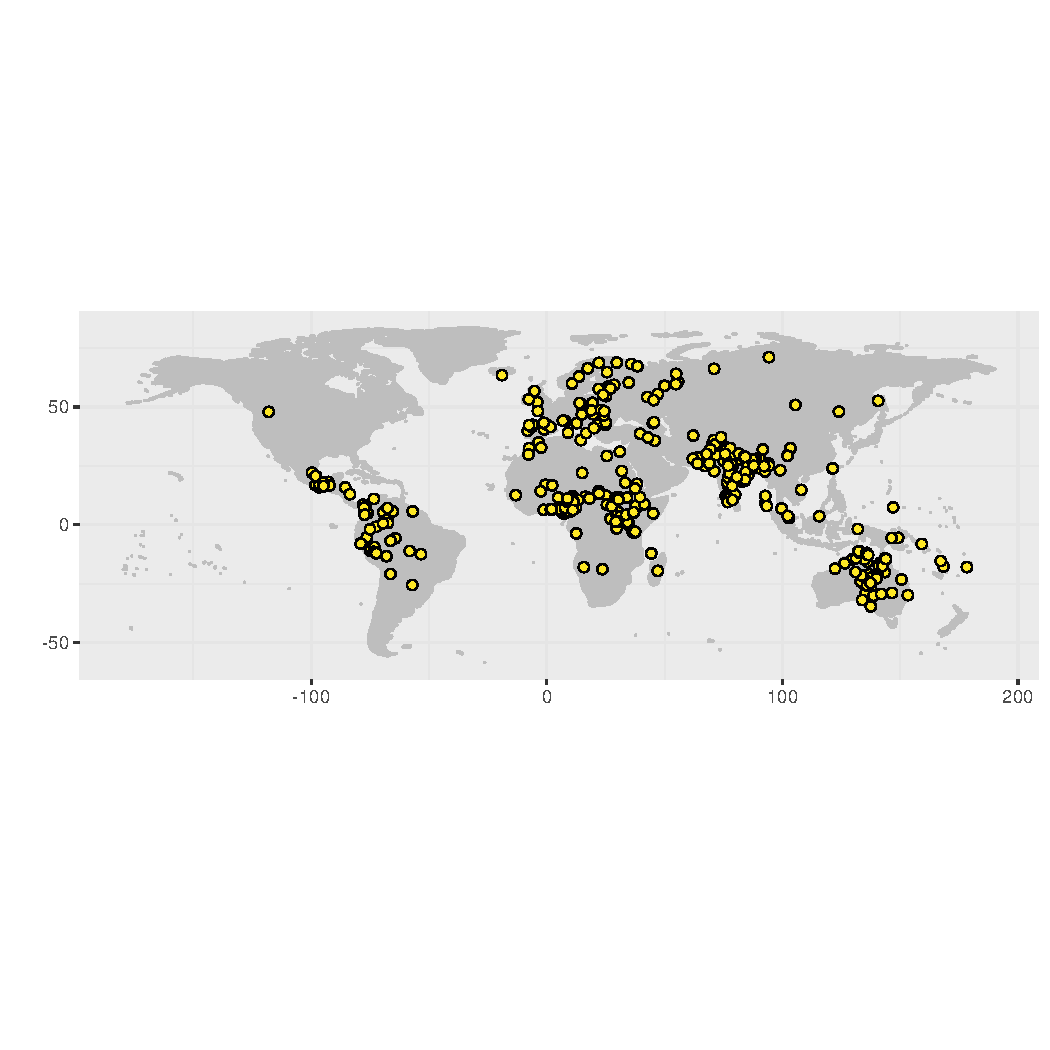
\includegraphics[width=1\linewidth,
	trim={0 5.65cm 0 5.25cm}, clip]{substance/images/contrast_lenght}
	\caption[Distribution de tous les contrastes de longueur des rhotiques dans les langues de PHOIBLE]{Distribution de tous les contrastes de longueur des rhotiques dans les langues de PHOIBLE selon les six critères de sélection de présence des segments dans les inventaires : /r/ en opposition à /ɾ/, /r/ en opposition à /rː/, /r/ en opposition à /ɽ/, /ɾ/ en opposition à /ɽ/, /ɾ/ en opposition à /ɾː/, /ɽ/ en opposition à /ɽː/. Il s'agit de langues où la présence des oppositions dans les rhotiques peut influencer positivement la présence des trills phonétiques. Chaque point jaune serait donc idéalement une langue avec un trill phonétique (ce qui n'est pas le cas dans les faits).}
	\label{fig:contrastlenght}
\end{figure}



%Nous ne nous intéressons pas au contraste mais bien à un facteur influençant la présence du trill.

Ces résultats sont aussi à mettre en perspective avec la réflexion de \textcite{labruneConsonnesRhotiquesGascon} sur le gascon, et sur les contrastes entre [ɾ] et [r]. Le gascon possède les deux phones qui sont interprétés comme deux allophones d'un seul phonème. Ainsi, en fonction de l'analyse de la langue, cela peut opacifier la réalité phonétique.\\

Le dernier exemple que nous avons présenté sur les contrastes de longueur dans les rhotiques nous a permis de mettre en évidence, une fois de plus, que travailler avec des grammaires n'est pas une tâche simple et qu'il faut être critique avec les représentations des sons à travers les symboles utilisés.

\section{Discussion}

Nous avions vu que de rapporter les sons d'une langue à partir d'une grammaire était complexe. Nous constatons que la recherche des trills dans ces ouvrages l'est tout autant.\\

Nous avons vu dans ce chapitre que le terrain en phonétique ainsi que la transcription des enregistrements sonores récoltés, requièrent énormément de connaissances et de compétences. 
Chaque langue est unique, par conséquent chaque grammaire est unique, ce qui explique les problèmes de comparabilité.\\

Des complications subsistent avec la multiplication des différents systèmes de transcriptions où le même symbole peut exister mais avec une valeur phonétique différente.
En ce qui concerne les rhotiques, dans beaucoup de cas, la présence du terme \textg{trill} dans une grammaire est suffisante pour dire que la langue décrite possède un trill. Cependant, à cause de toute la variation qu'englobe le trill de l'acoustique à l'inventaire phonémique, il faut plus qu'un label descriptif pour convaincre que la réalisation du trill est bien trillée. Les grammaires tendent à réduire la variation phonétique à la représentation d'un phonème. 
Dans certains cas où le trill est mentionné, les exemples de \textg{palatalisation} et de \textg{nasalisation} mettent en évidence qu'il ne peut s'agir du trill, puisqu'il est articulatoirement défavorisé voire impossible.\\

Finalement, les grammaires sont utiles pour de nombreuses questions de recherche, mais tant qu'elles ne représenteront pas mieux la variation dans les rhotiques, elles ne seront pas une source fiable pour faire une typologie des trills.


